\chapter{Graphene nanoribbons}
The band structure of graphene nanoribbons is determined by the nature of their edges: armchair or zigzag. In figure \ref{fig:edges} there is a piece of honeycomb lattice, which have zigzag edges along $x$ direction and armchair edge along the $y$ direction. 
\begin{figure}[h] 
\begin{center}
  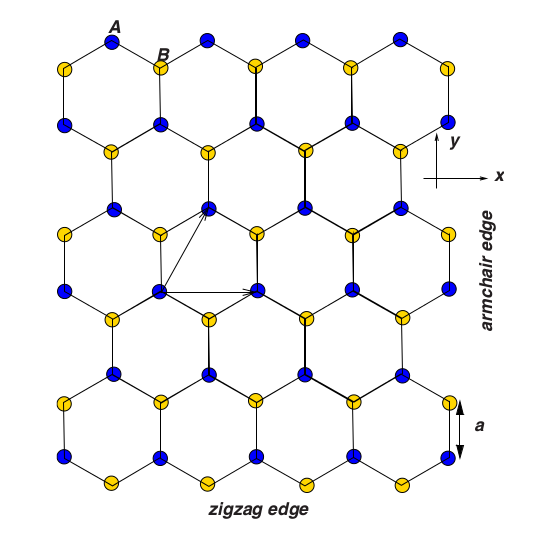
\includegraphics[width=0.3\linewidth]{img/nanoribbbon_edges}
  \caption{A piece of honeycomb lattice with both zigzag and armchair edges. \label{fig:edges}}
\end{center}
\end{figure}


\section{Armchair nanoribbons}
Armchair nanoribbons can have either metallic or semiconducting character, depending on their width. In the TB calculations metallic armchair nanoribbons have energy bands crossing with linear dispersion. In fig. \ref{fig:ac_ribbons}
I show calculated band structures for a set of ribbons with different widths. Nanoribbons of widths $n= 11$ (fig. \ref{fig:ac11}) and $n=32$ (fig. \ref{fig:ac32}) have zero energy gap. However, DFT calculations show that armchair nanoribbons have non-zero energy gap scaling with the inverse of the ribbon width \cite{han}.
\begin{figure}[hb!]
\centering
\begin{subfigure}{.5\textwidth}
  \centering
  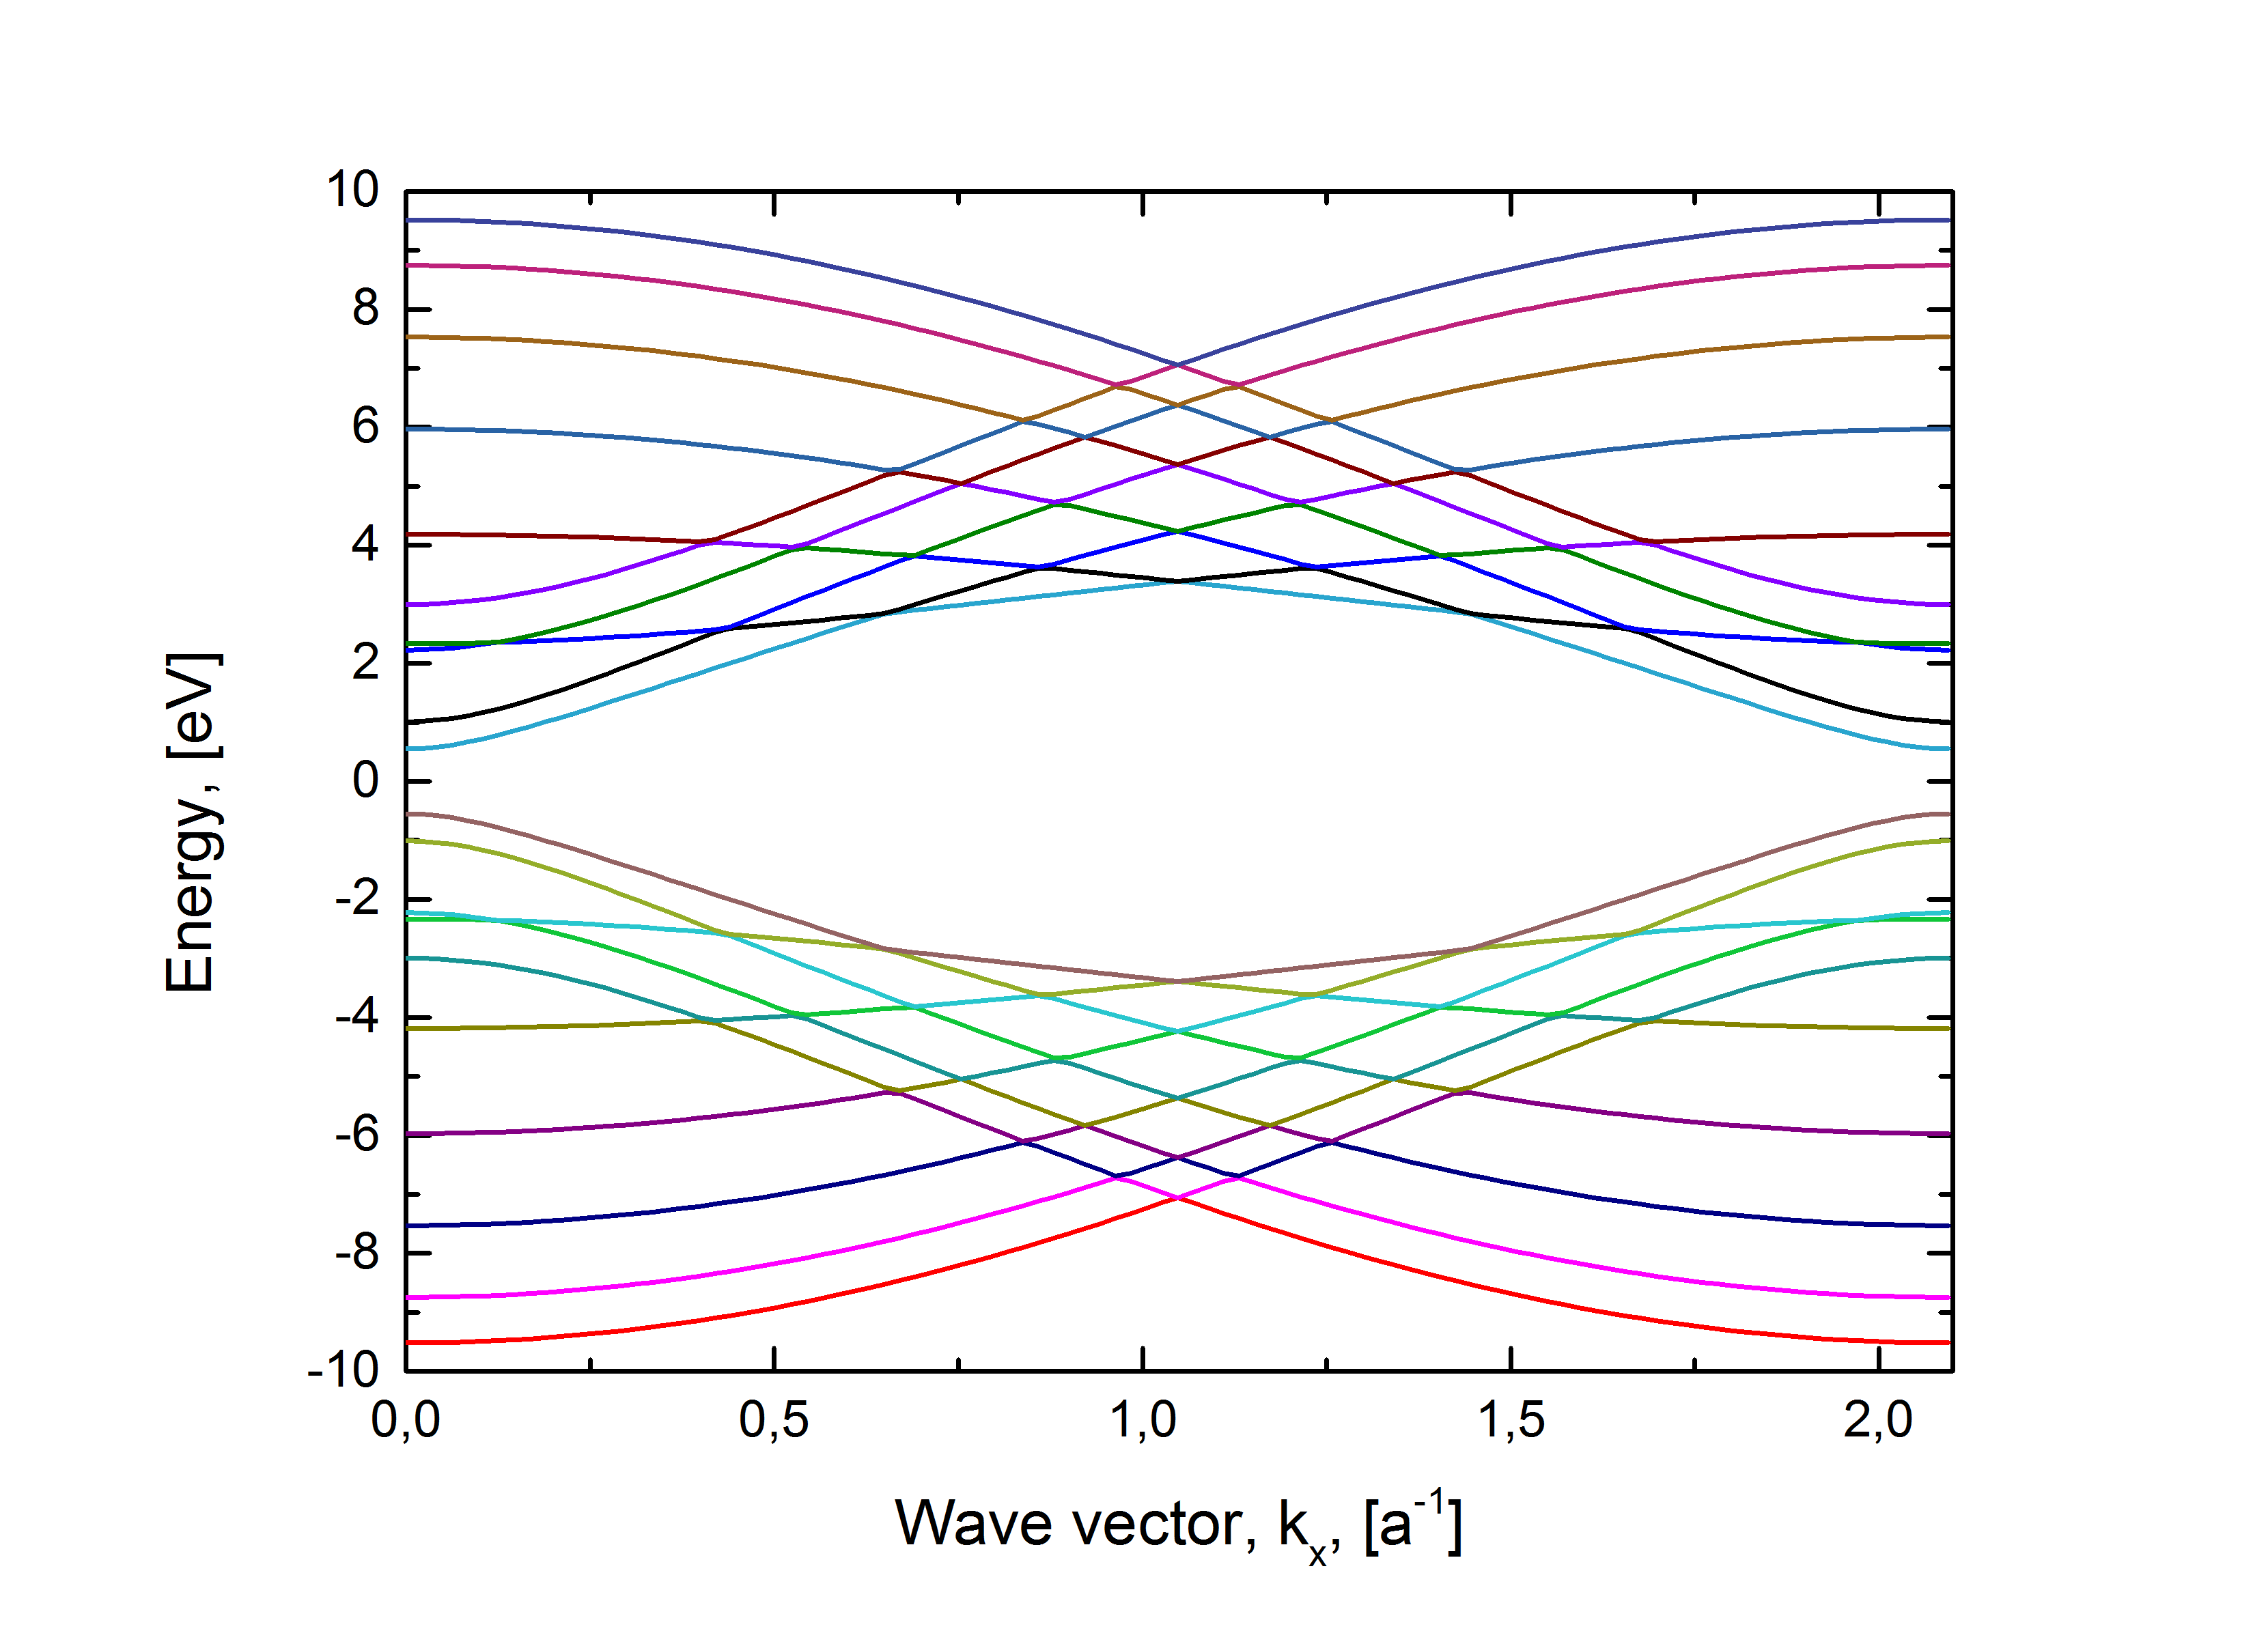
\includegraphics[width=\linewidth]{img/ac_ribbon_10}
  \caption{$n=10$}
  \label{fig:ac10}
\end{subfigure}%
\begin{subfigure}{.5\textwidth}
  \centering
  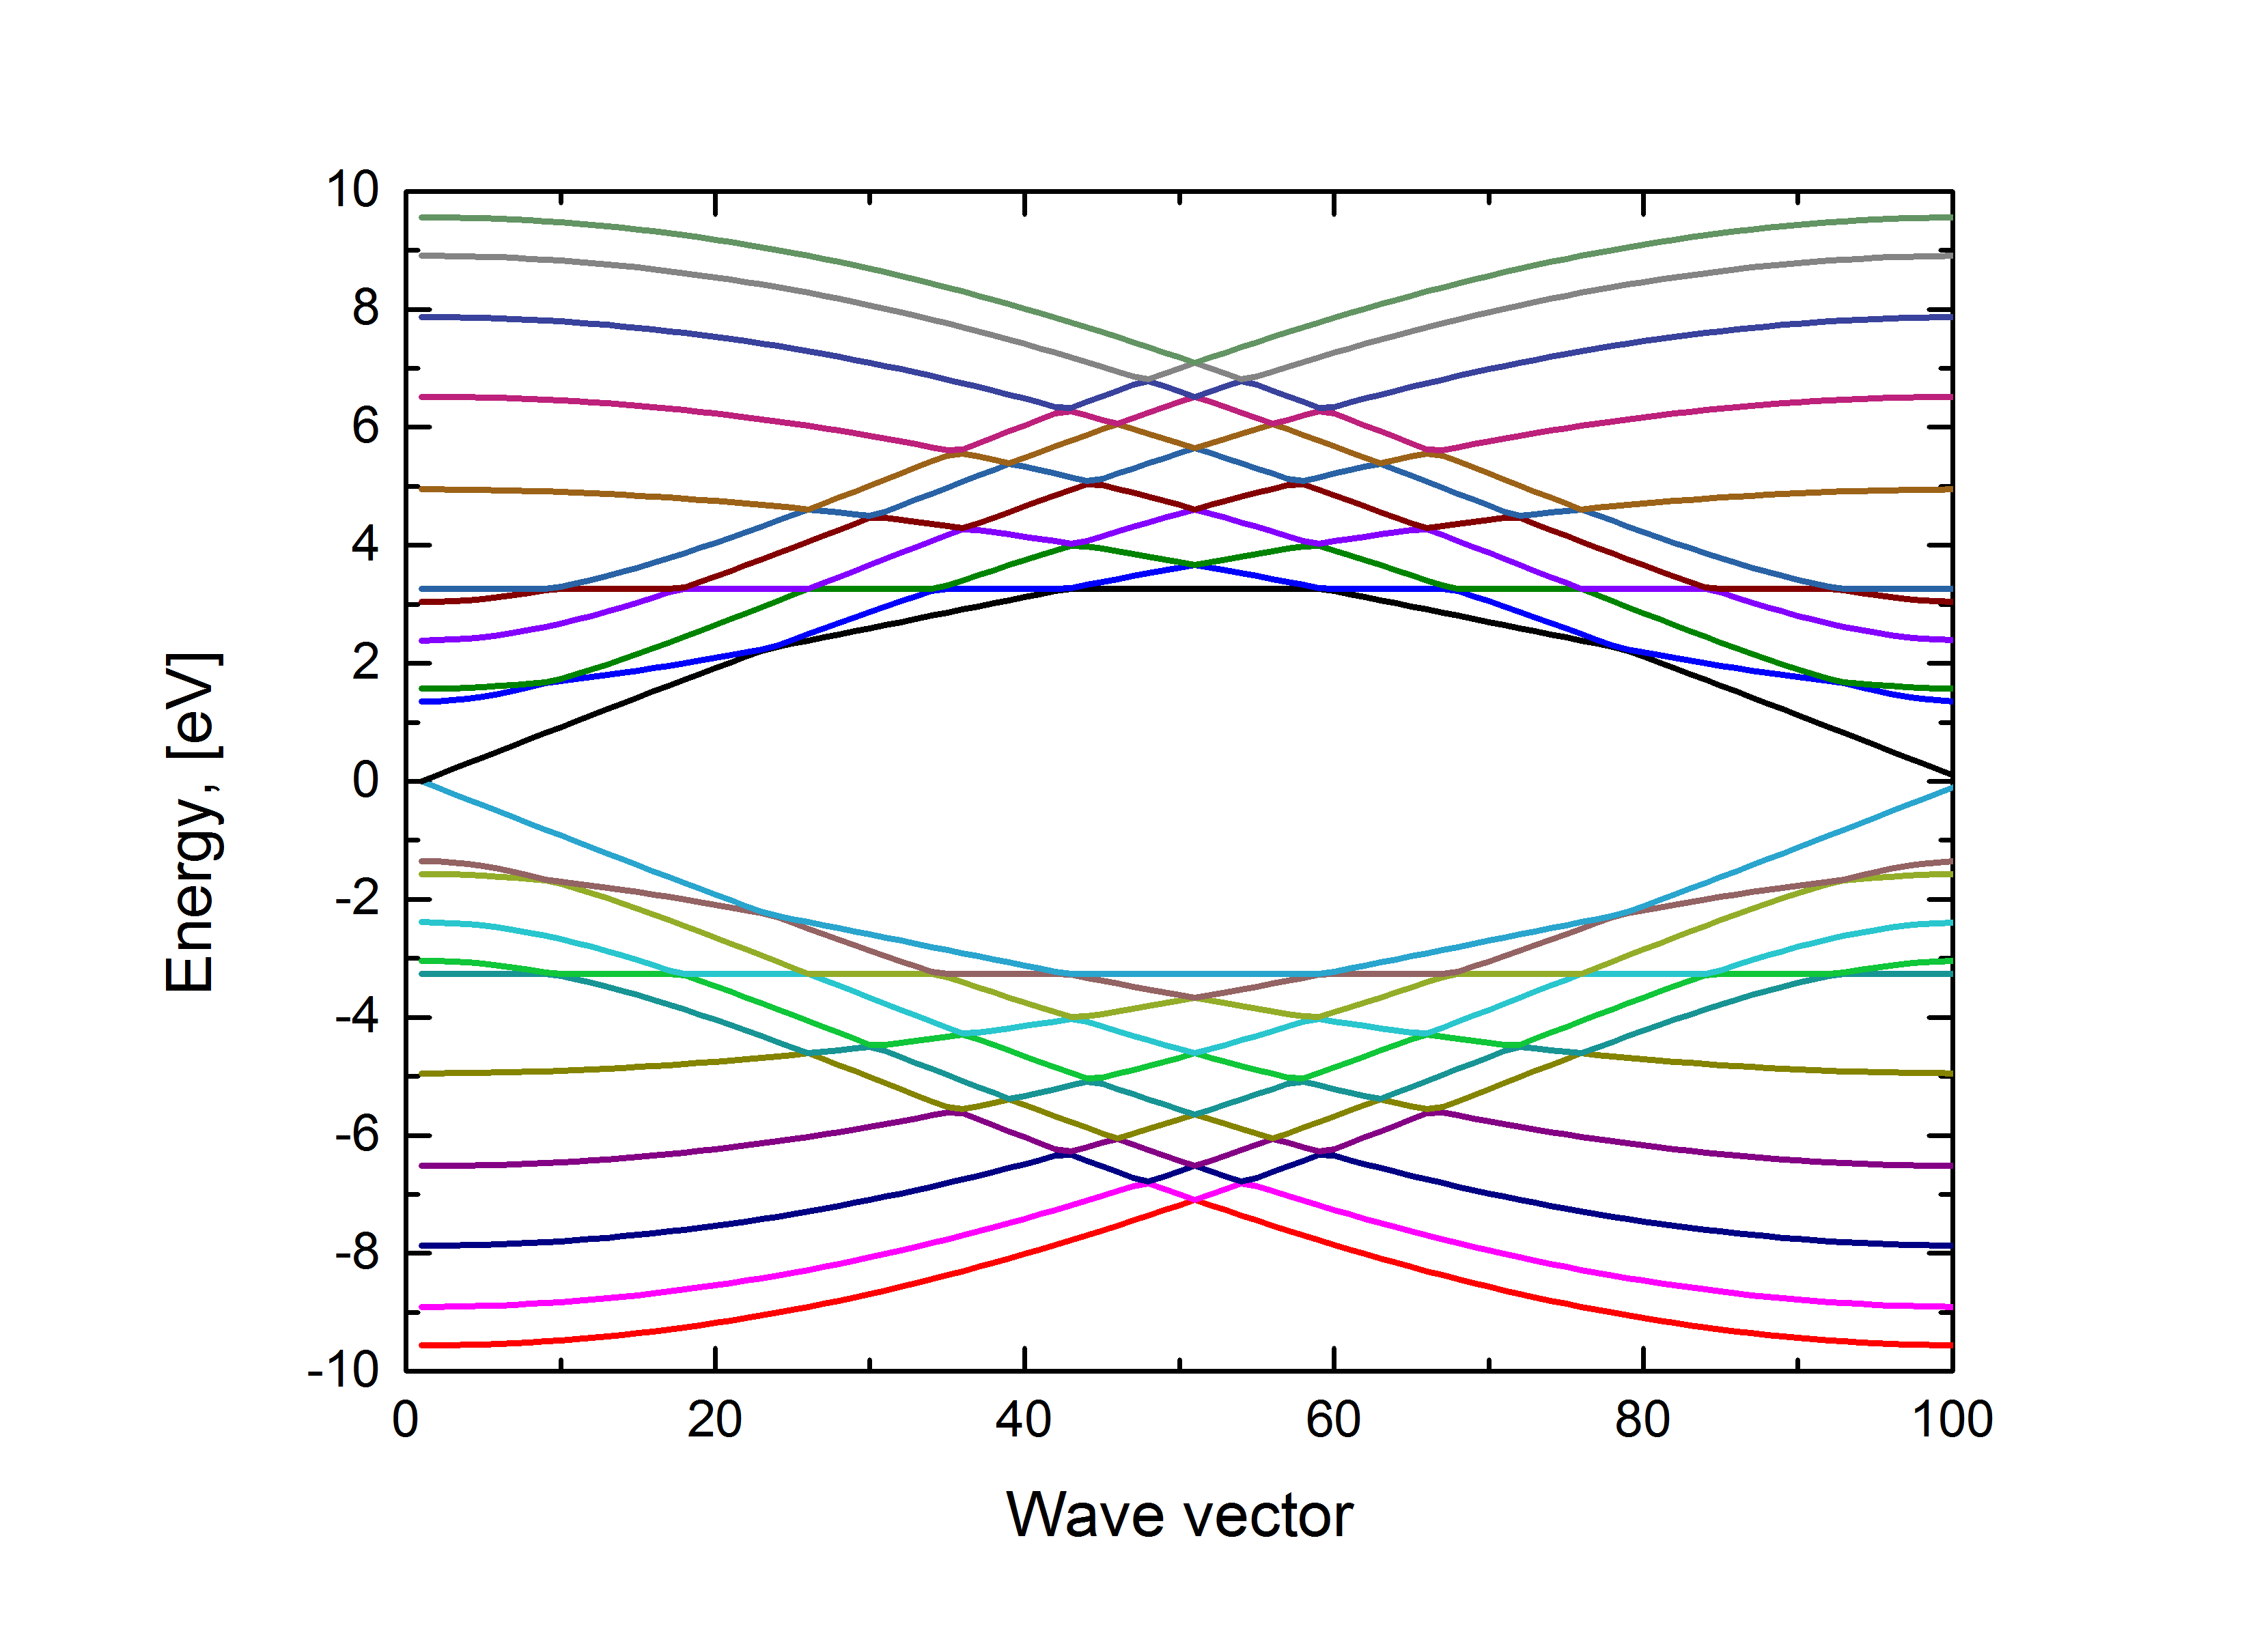
\includegraphics[width=\linewidth]{img/ac_ribbon_11}
  \caption{$n=11$}
  \label{fig:ac11}
\end{subfigure}
\begin{subfigure}{.5\textwidth}
  \centering
  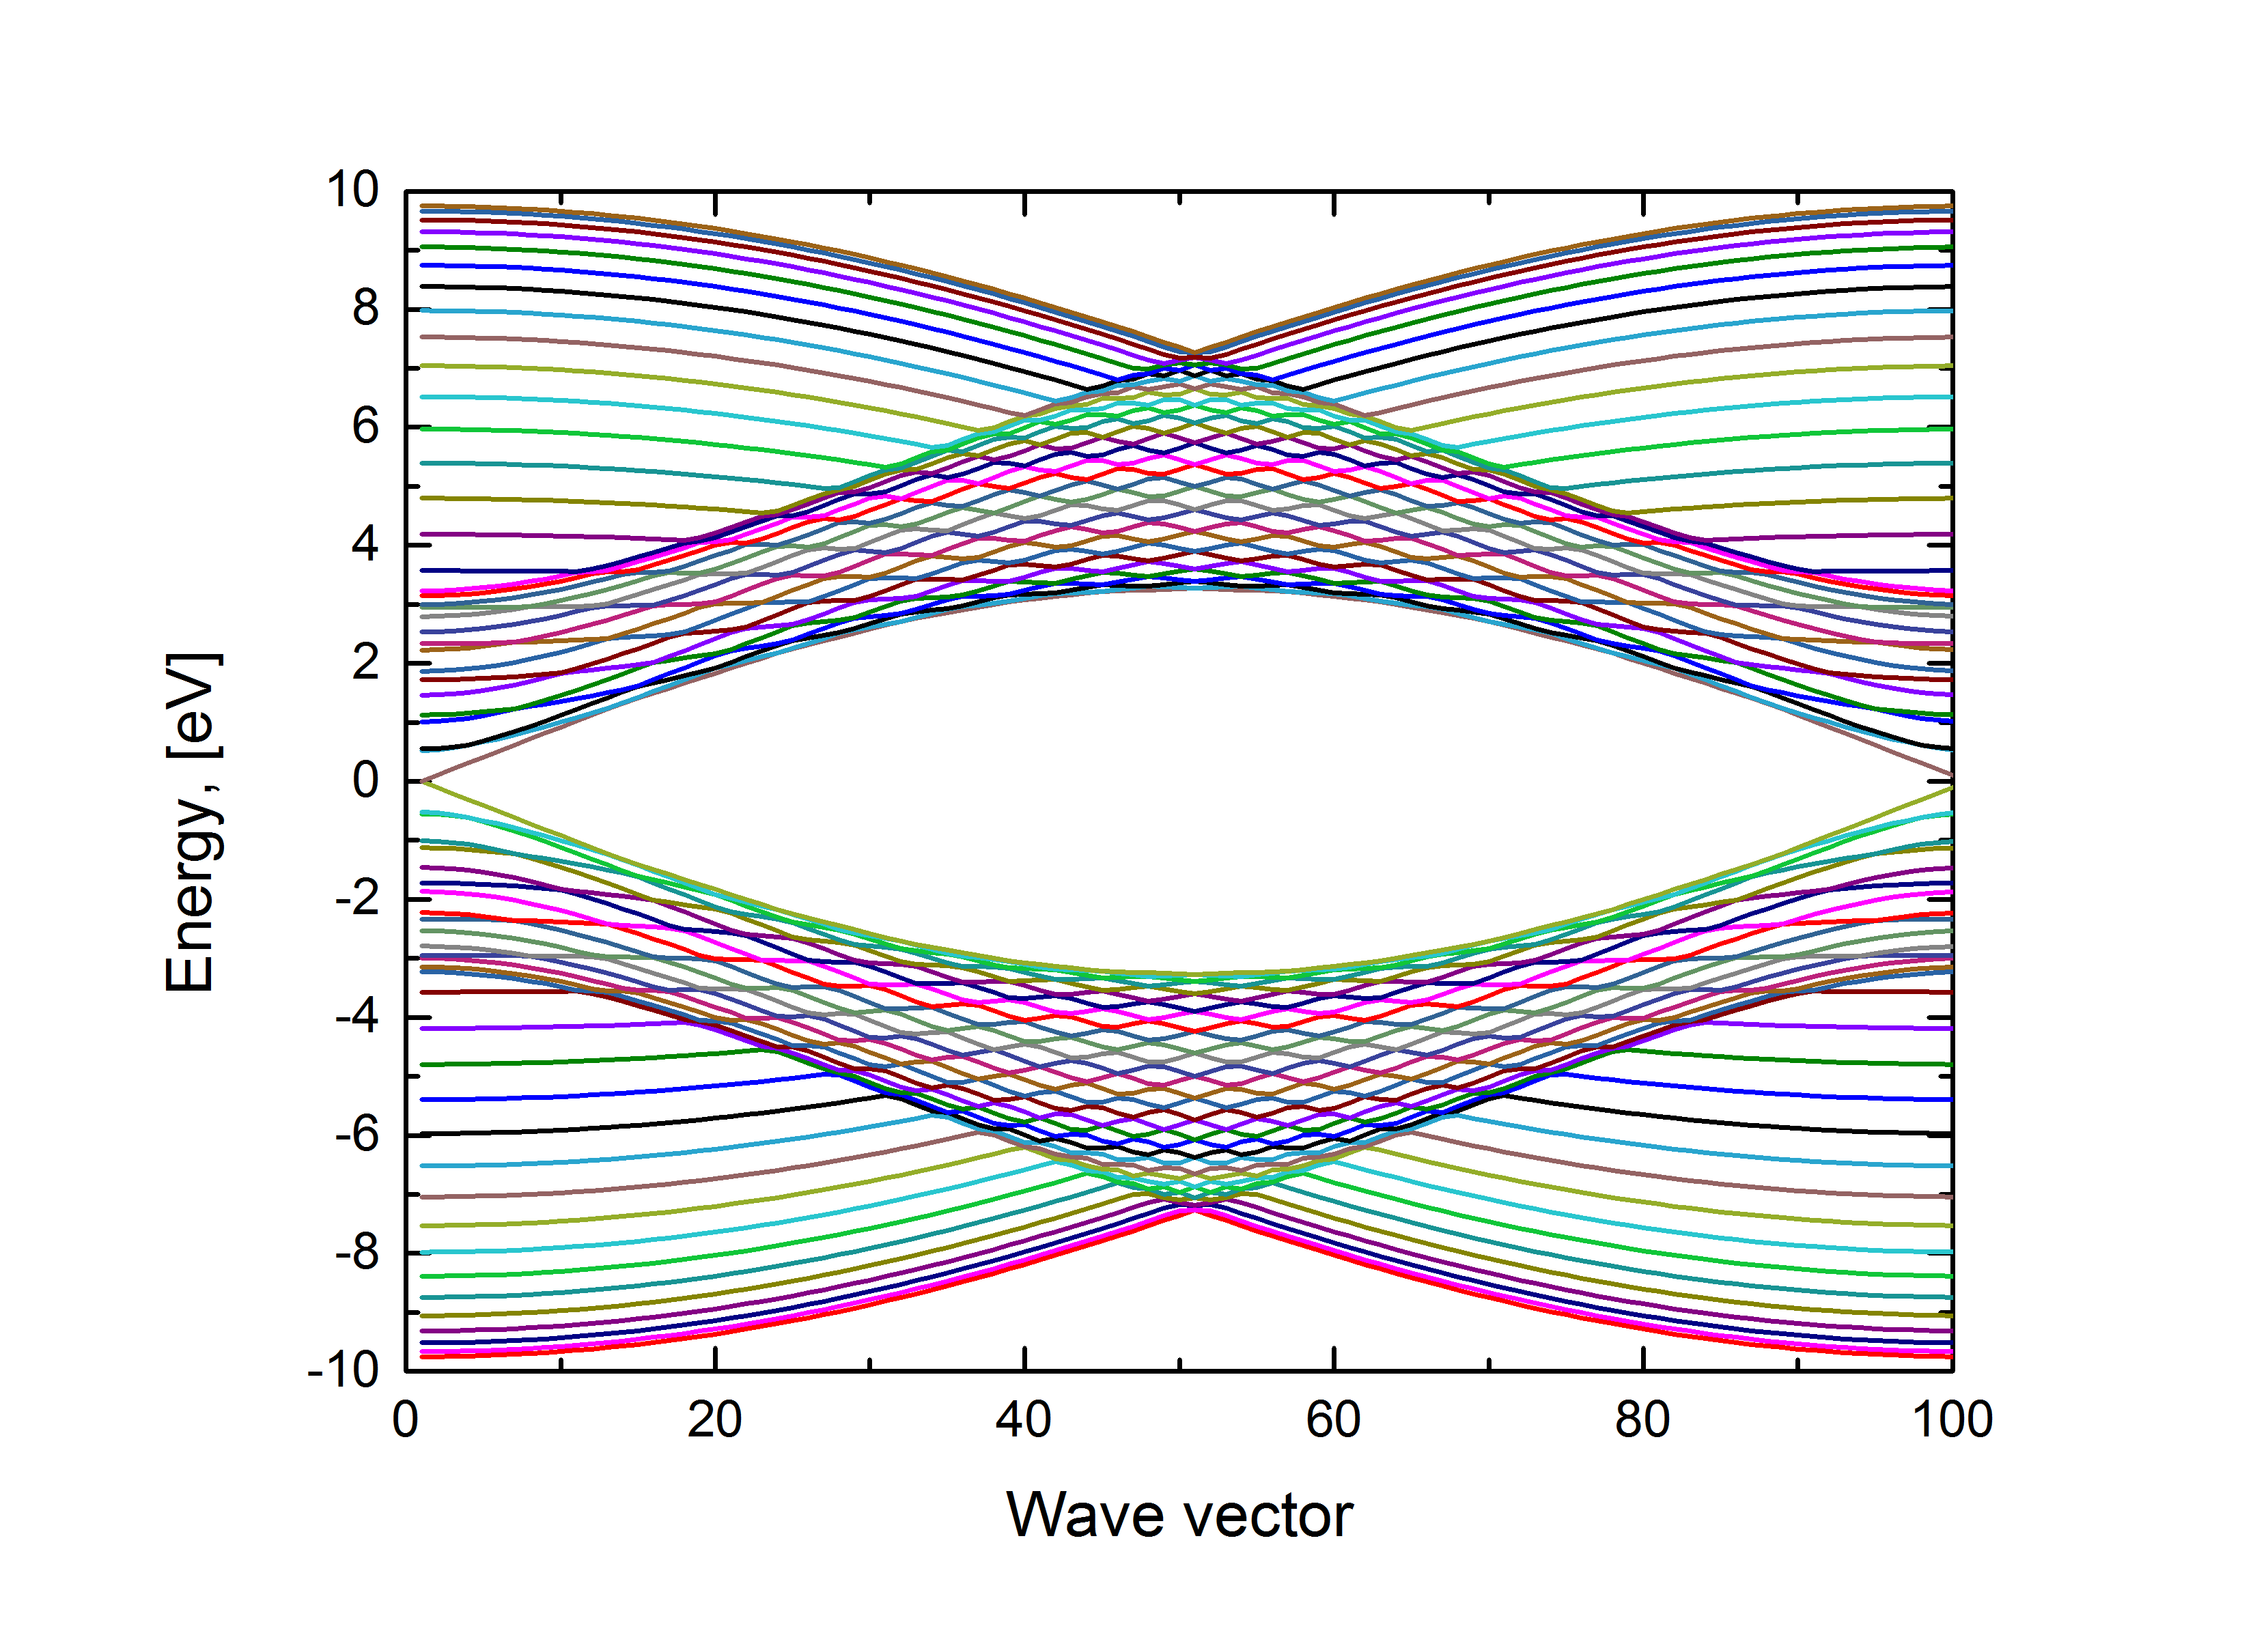
\includegraphics[width=\linewidth]{img/ac_ribbon_32}
  \caption{$n=32$}
  \label{fig:ac32}
\end{subfigure}%
\begin{subfigure}{.5\textwidth}
  \centering
  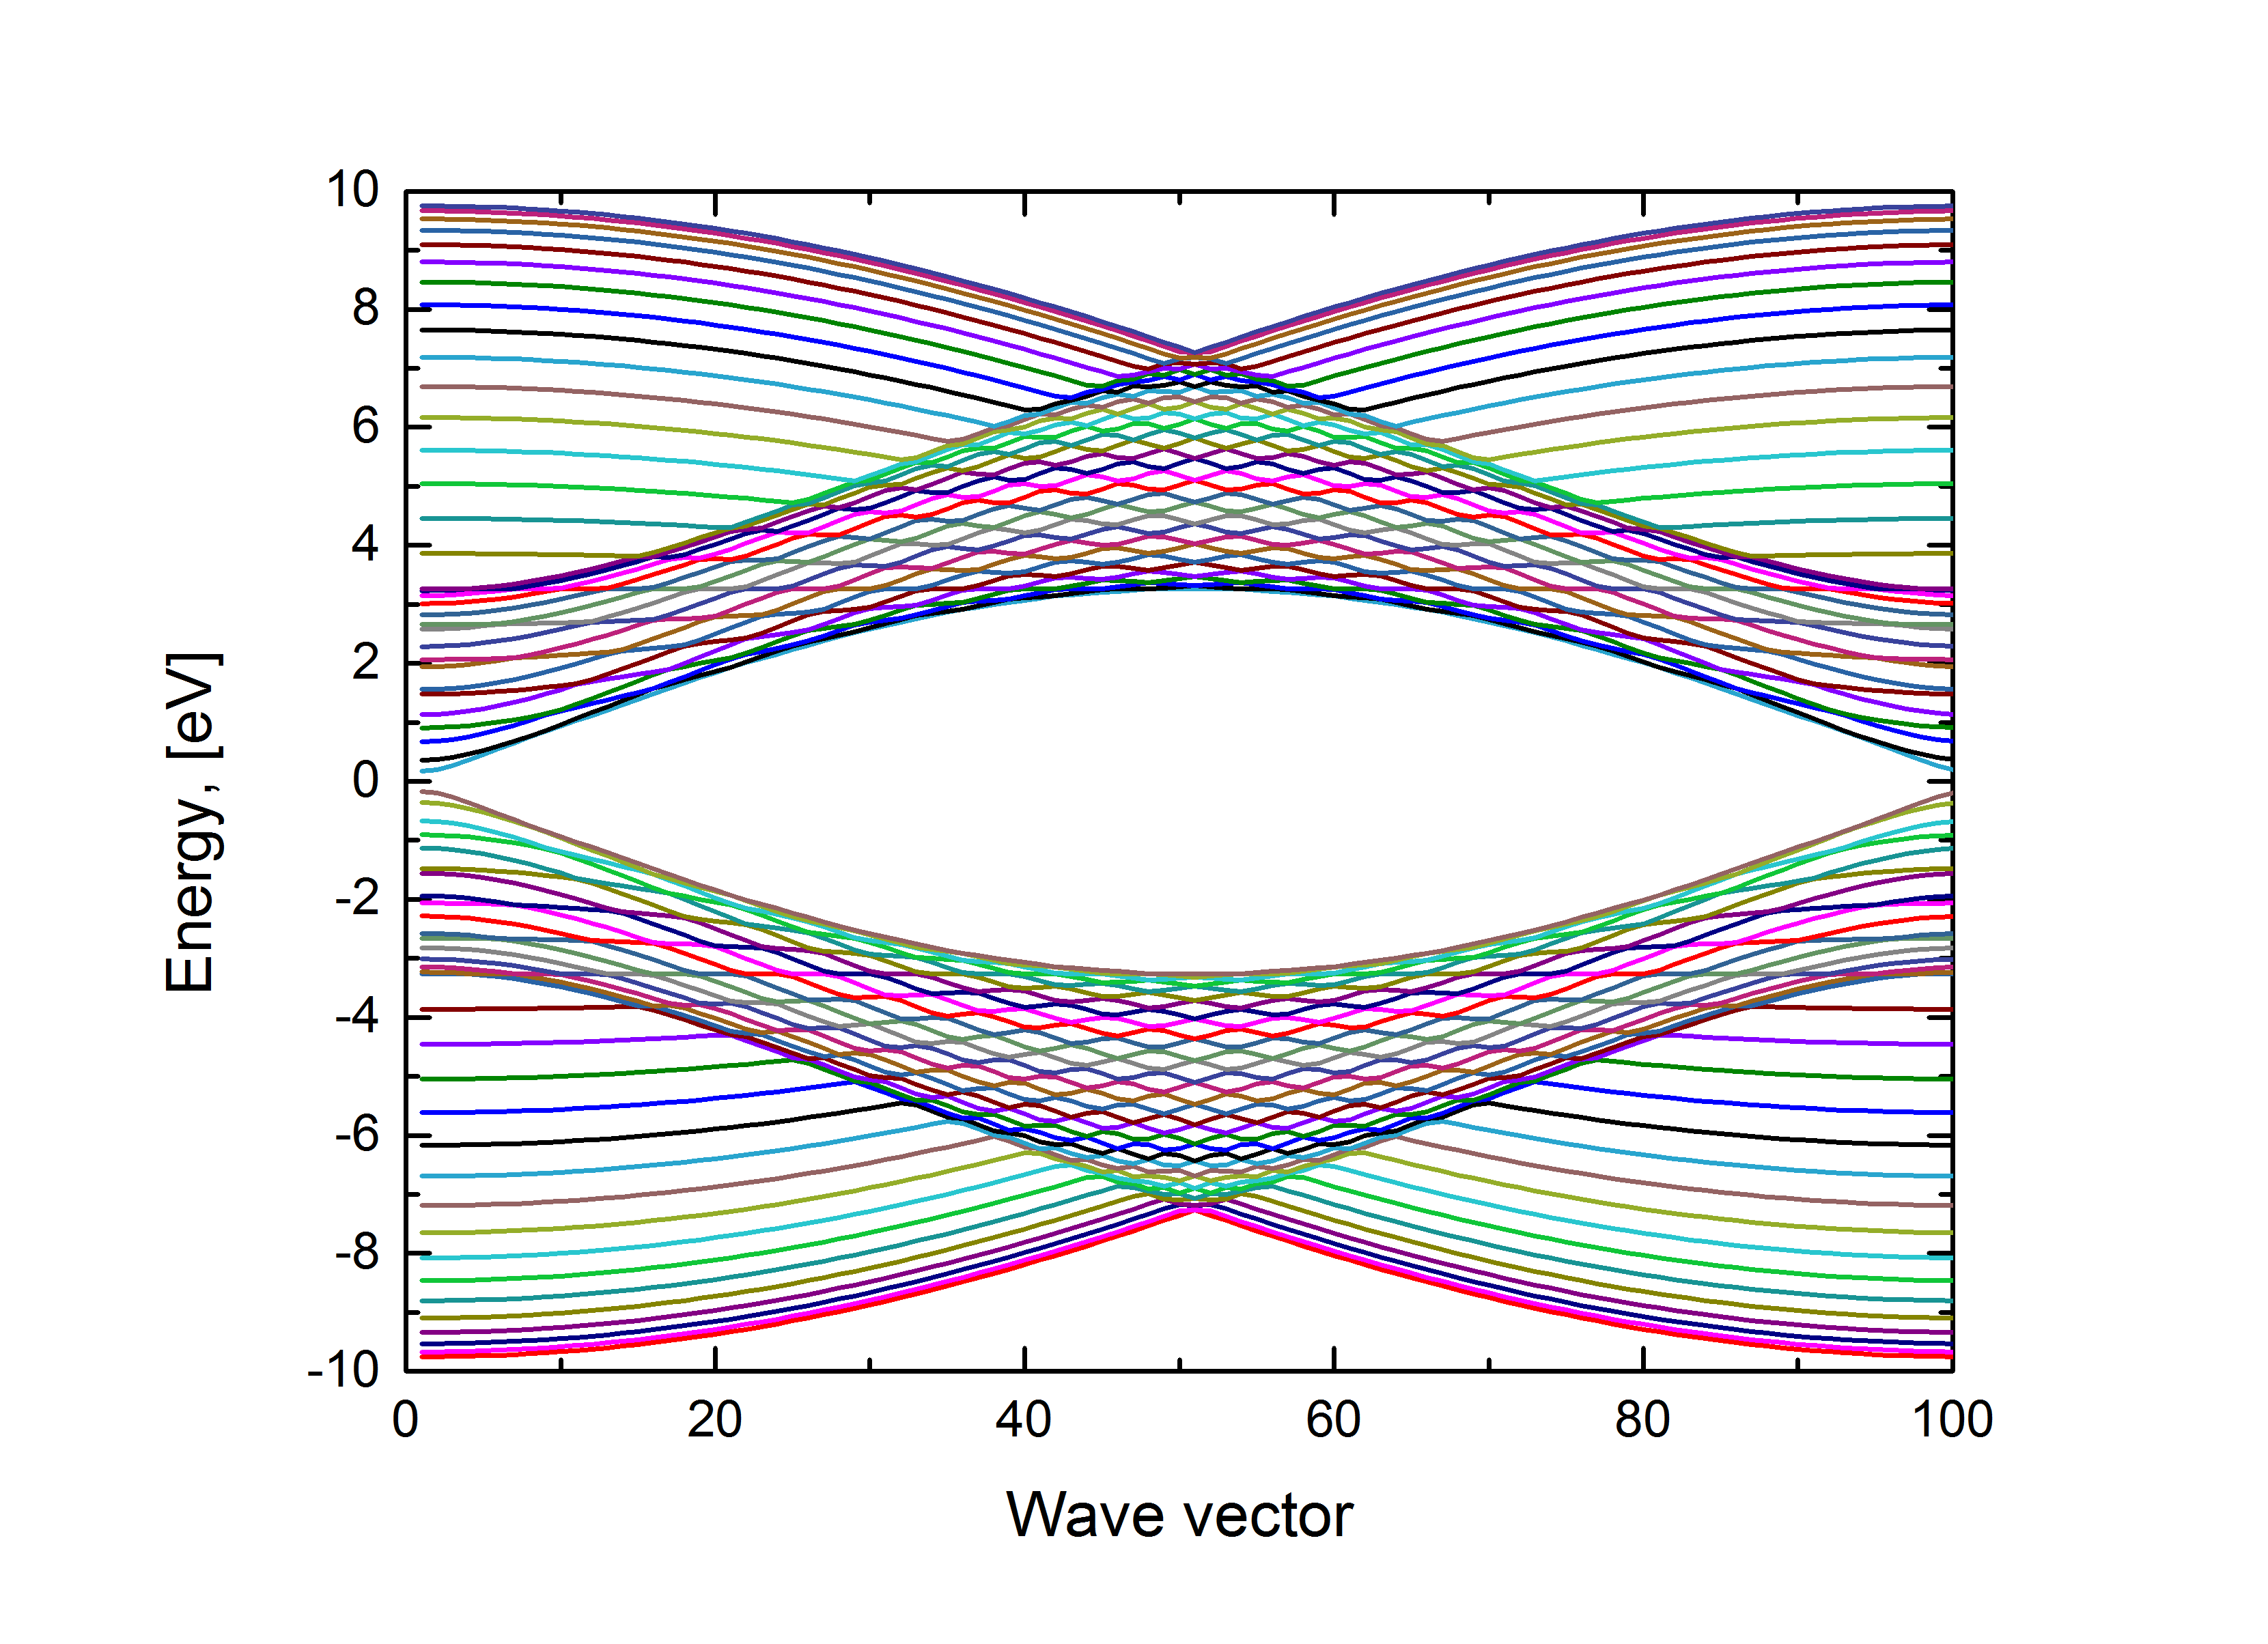
\includegraphics[width=\linewidth]{img/ac_ribbon_33}
  \caption{$n=33$}
  \label{fig:ac33}
\end{subfigure}
\begin{subfigure}{.5\textwidth}
  \centering
  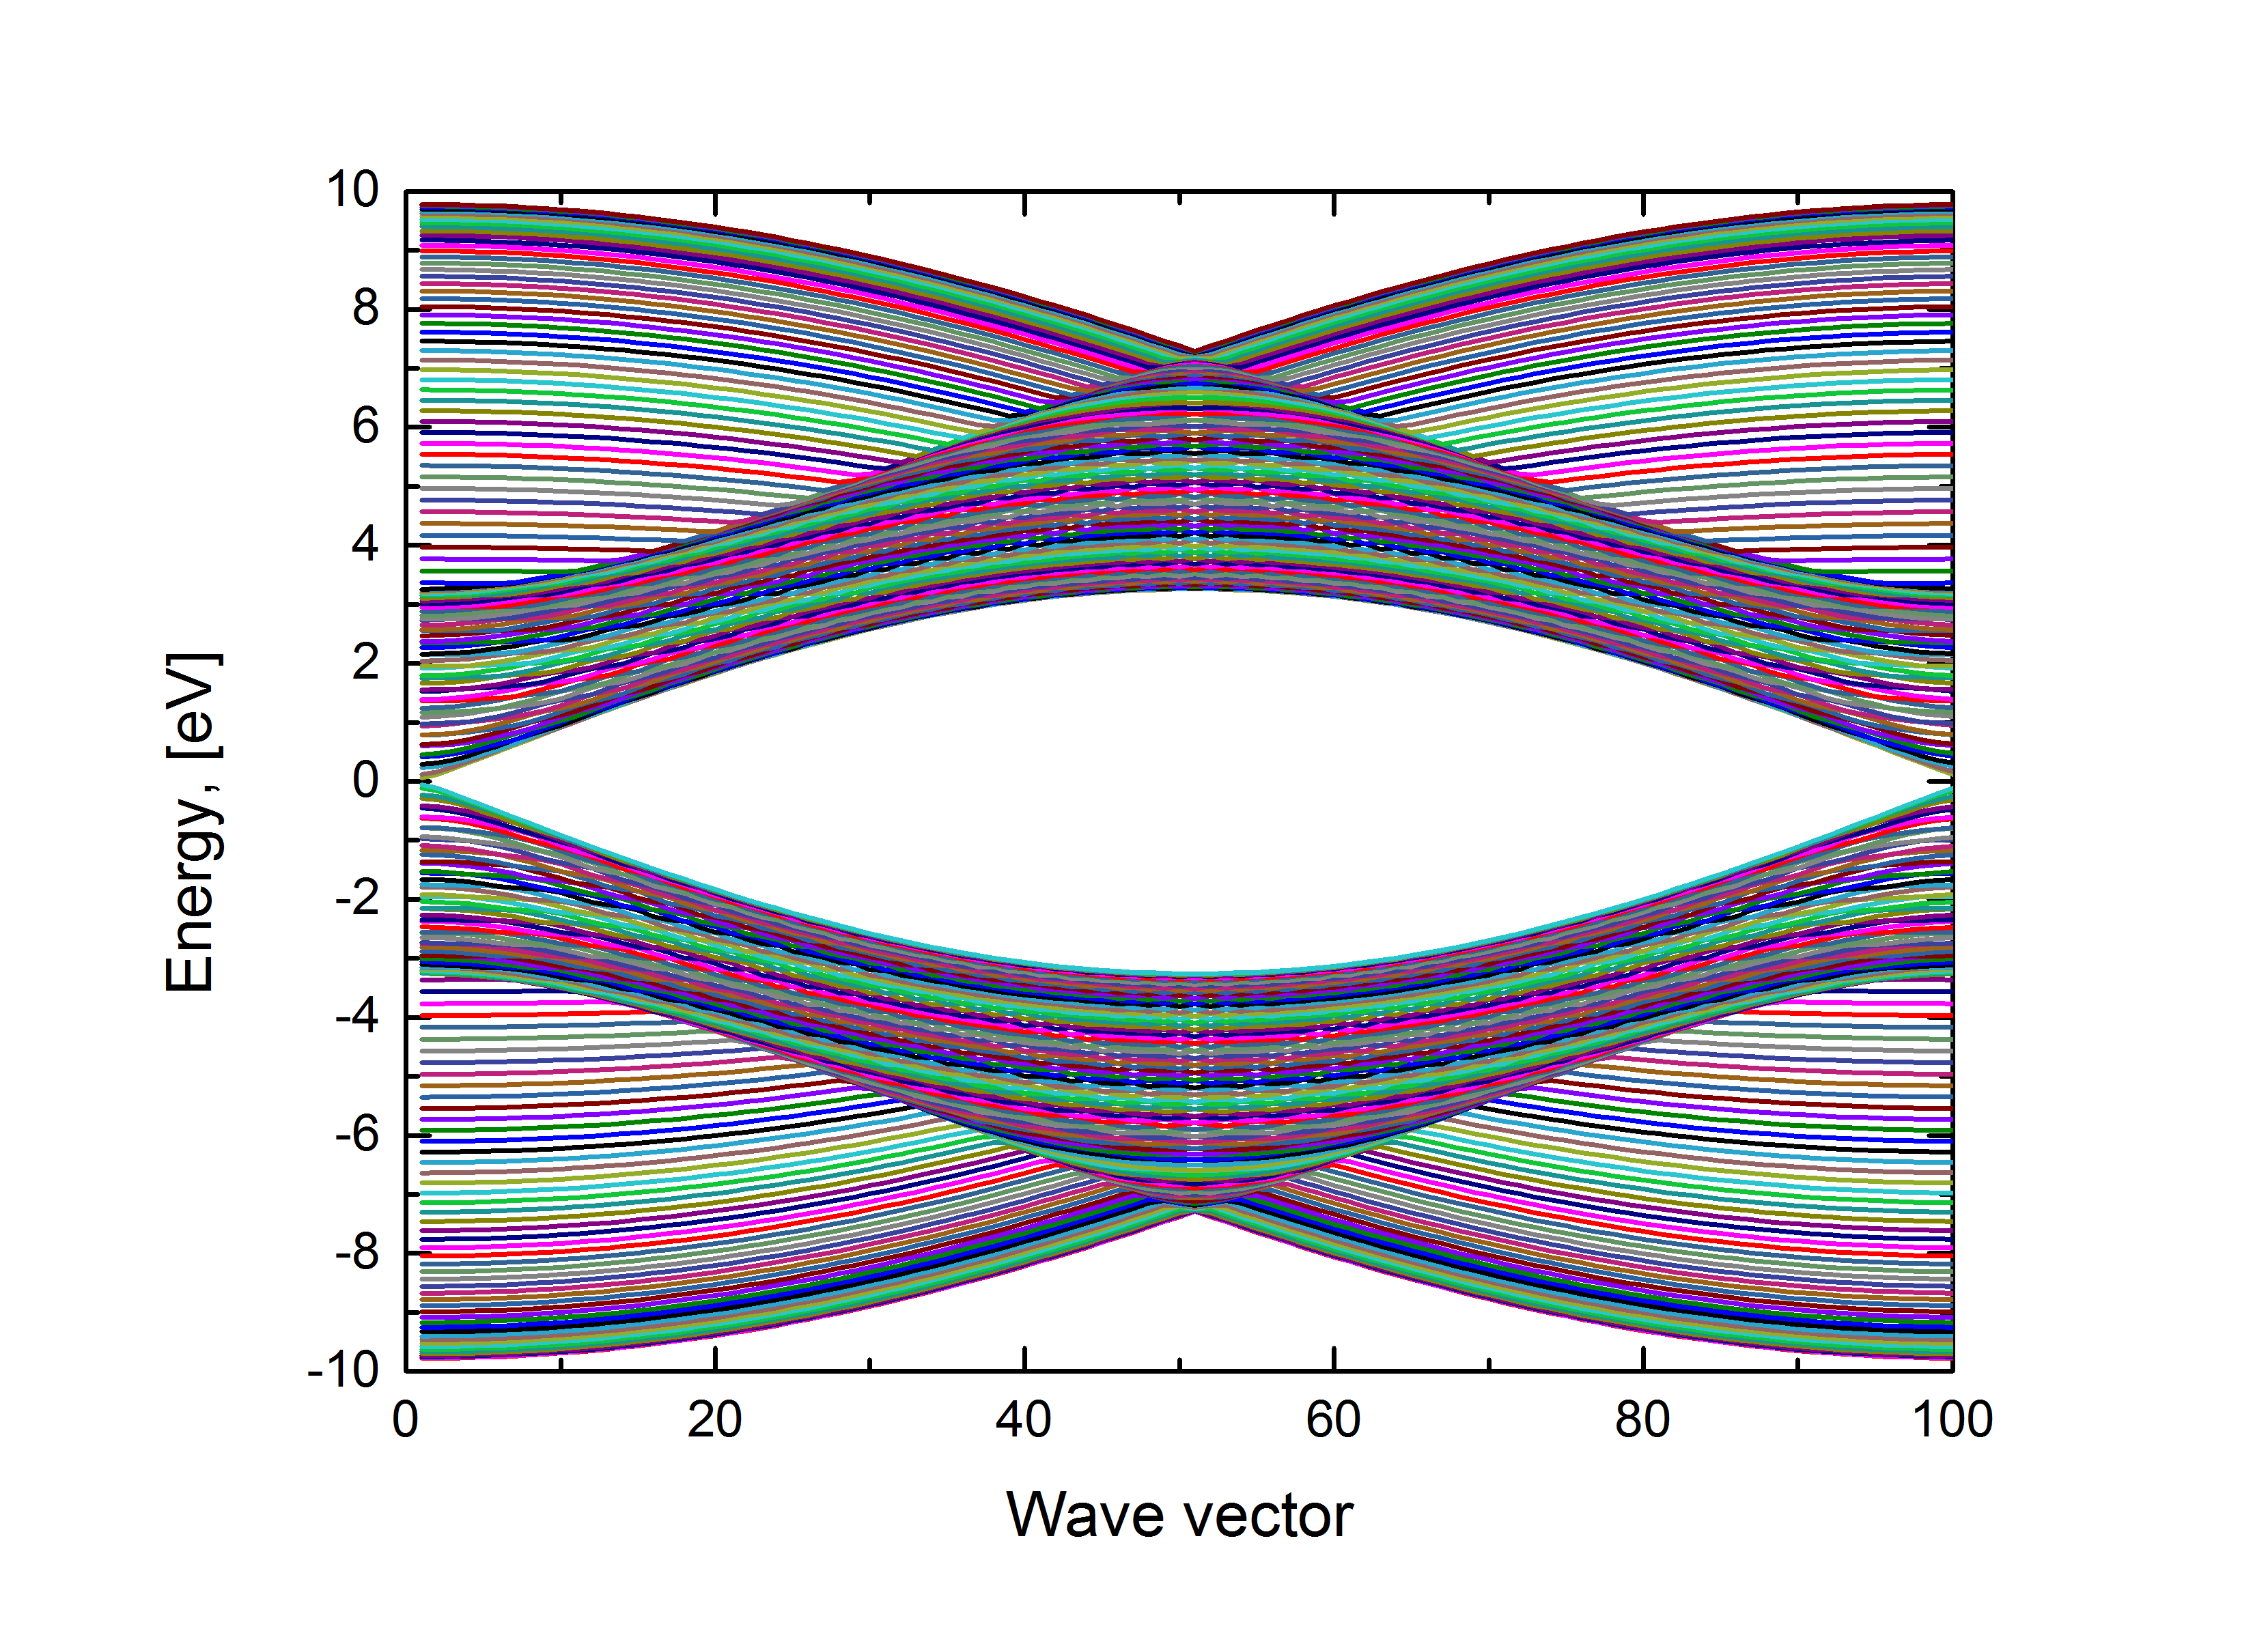
\includegraphics[width=\linewidth]{img/ac_ribbon_100}
  \caption{$n=100$}
  \label{fig:ac100}
\end{subfigure}
\caption{Calculated band structure of armchair nanoribbons of various widths $n$ atoms. \label{fig:ac_ribbons}}
\end{figure}

\section{Zigzag nanoribbons}
In TB model calculations zigzag nanoribbons are always metallic and have a zero-energy band. This dispersionless zero-energy mode is the surface states confined near the edge of the graphene ribbon. However in the experiments graphene nanoribbons are highly disordered at the edges \cite{areshkin} and often passivated by hydrogen \cite{barone}. All these strongly effect the properties of edge states. On fig. \ref{fig:zz_ribbons} I show calculated spectrum of zigzag graphene nanoribbons of various widths.
\begin{figure}[hb!]
\centering
\begin{subfigure}{.5\textwidth}
  \centering
  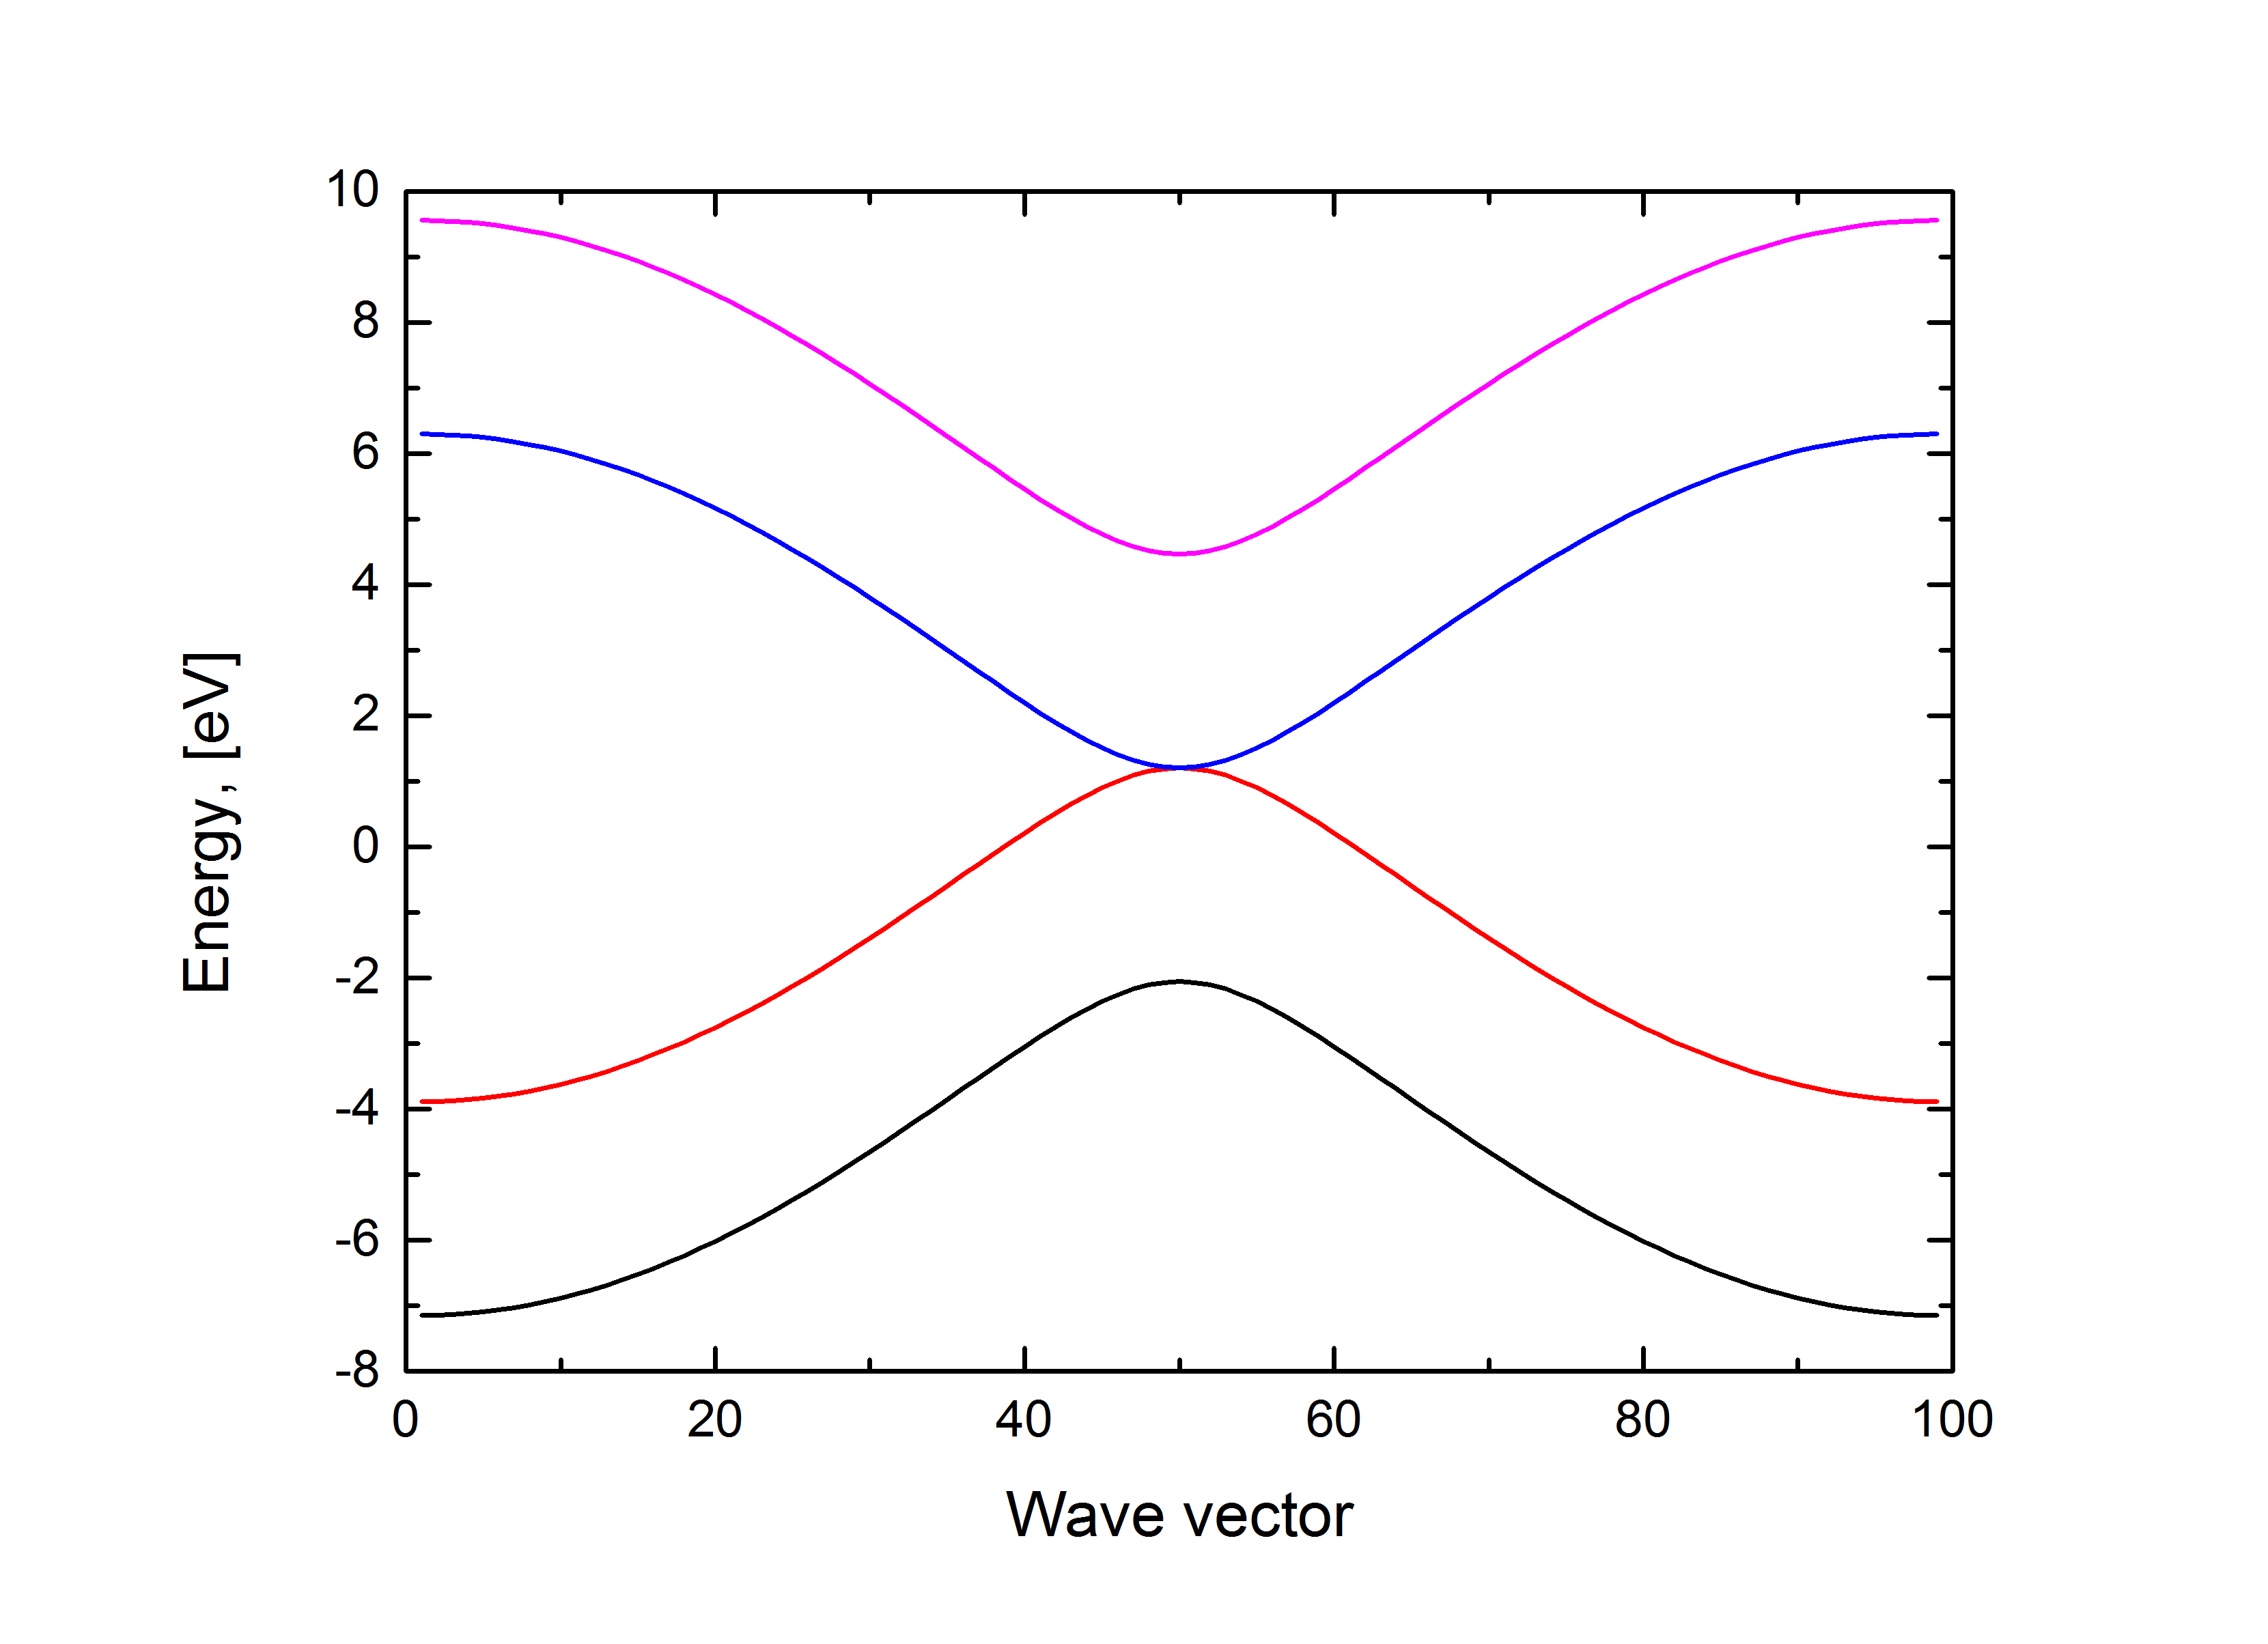
\includegraphics[width=\linewidth]{img/zz_ribbon_2}
  \caption{$n=2$}
  \label{fig:zz2}
\end{subfigure}%
\begin{subfigure}{.5\textwidth}
  \centering
  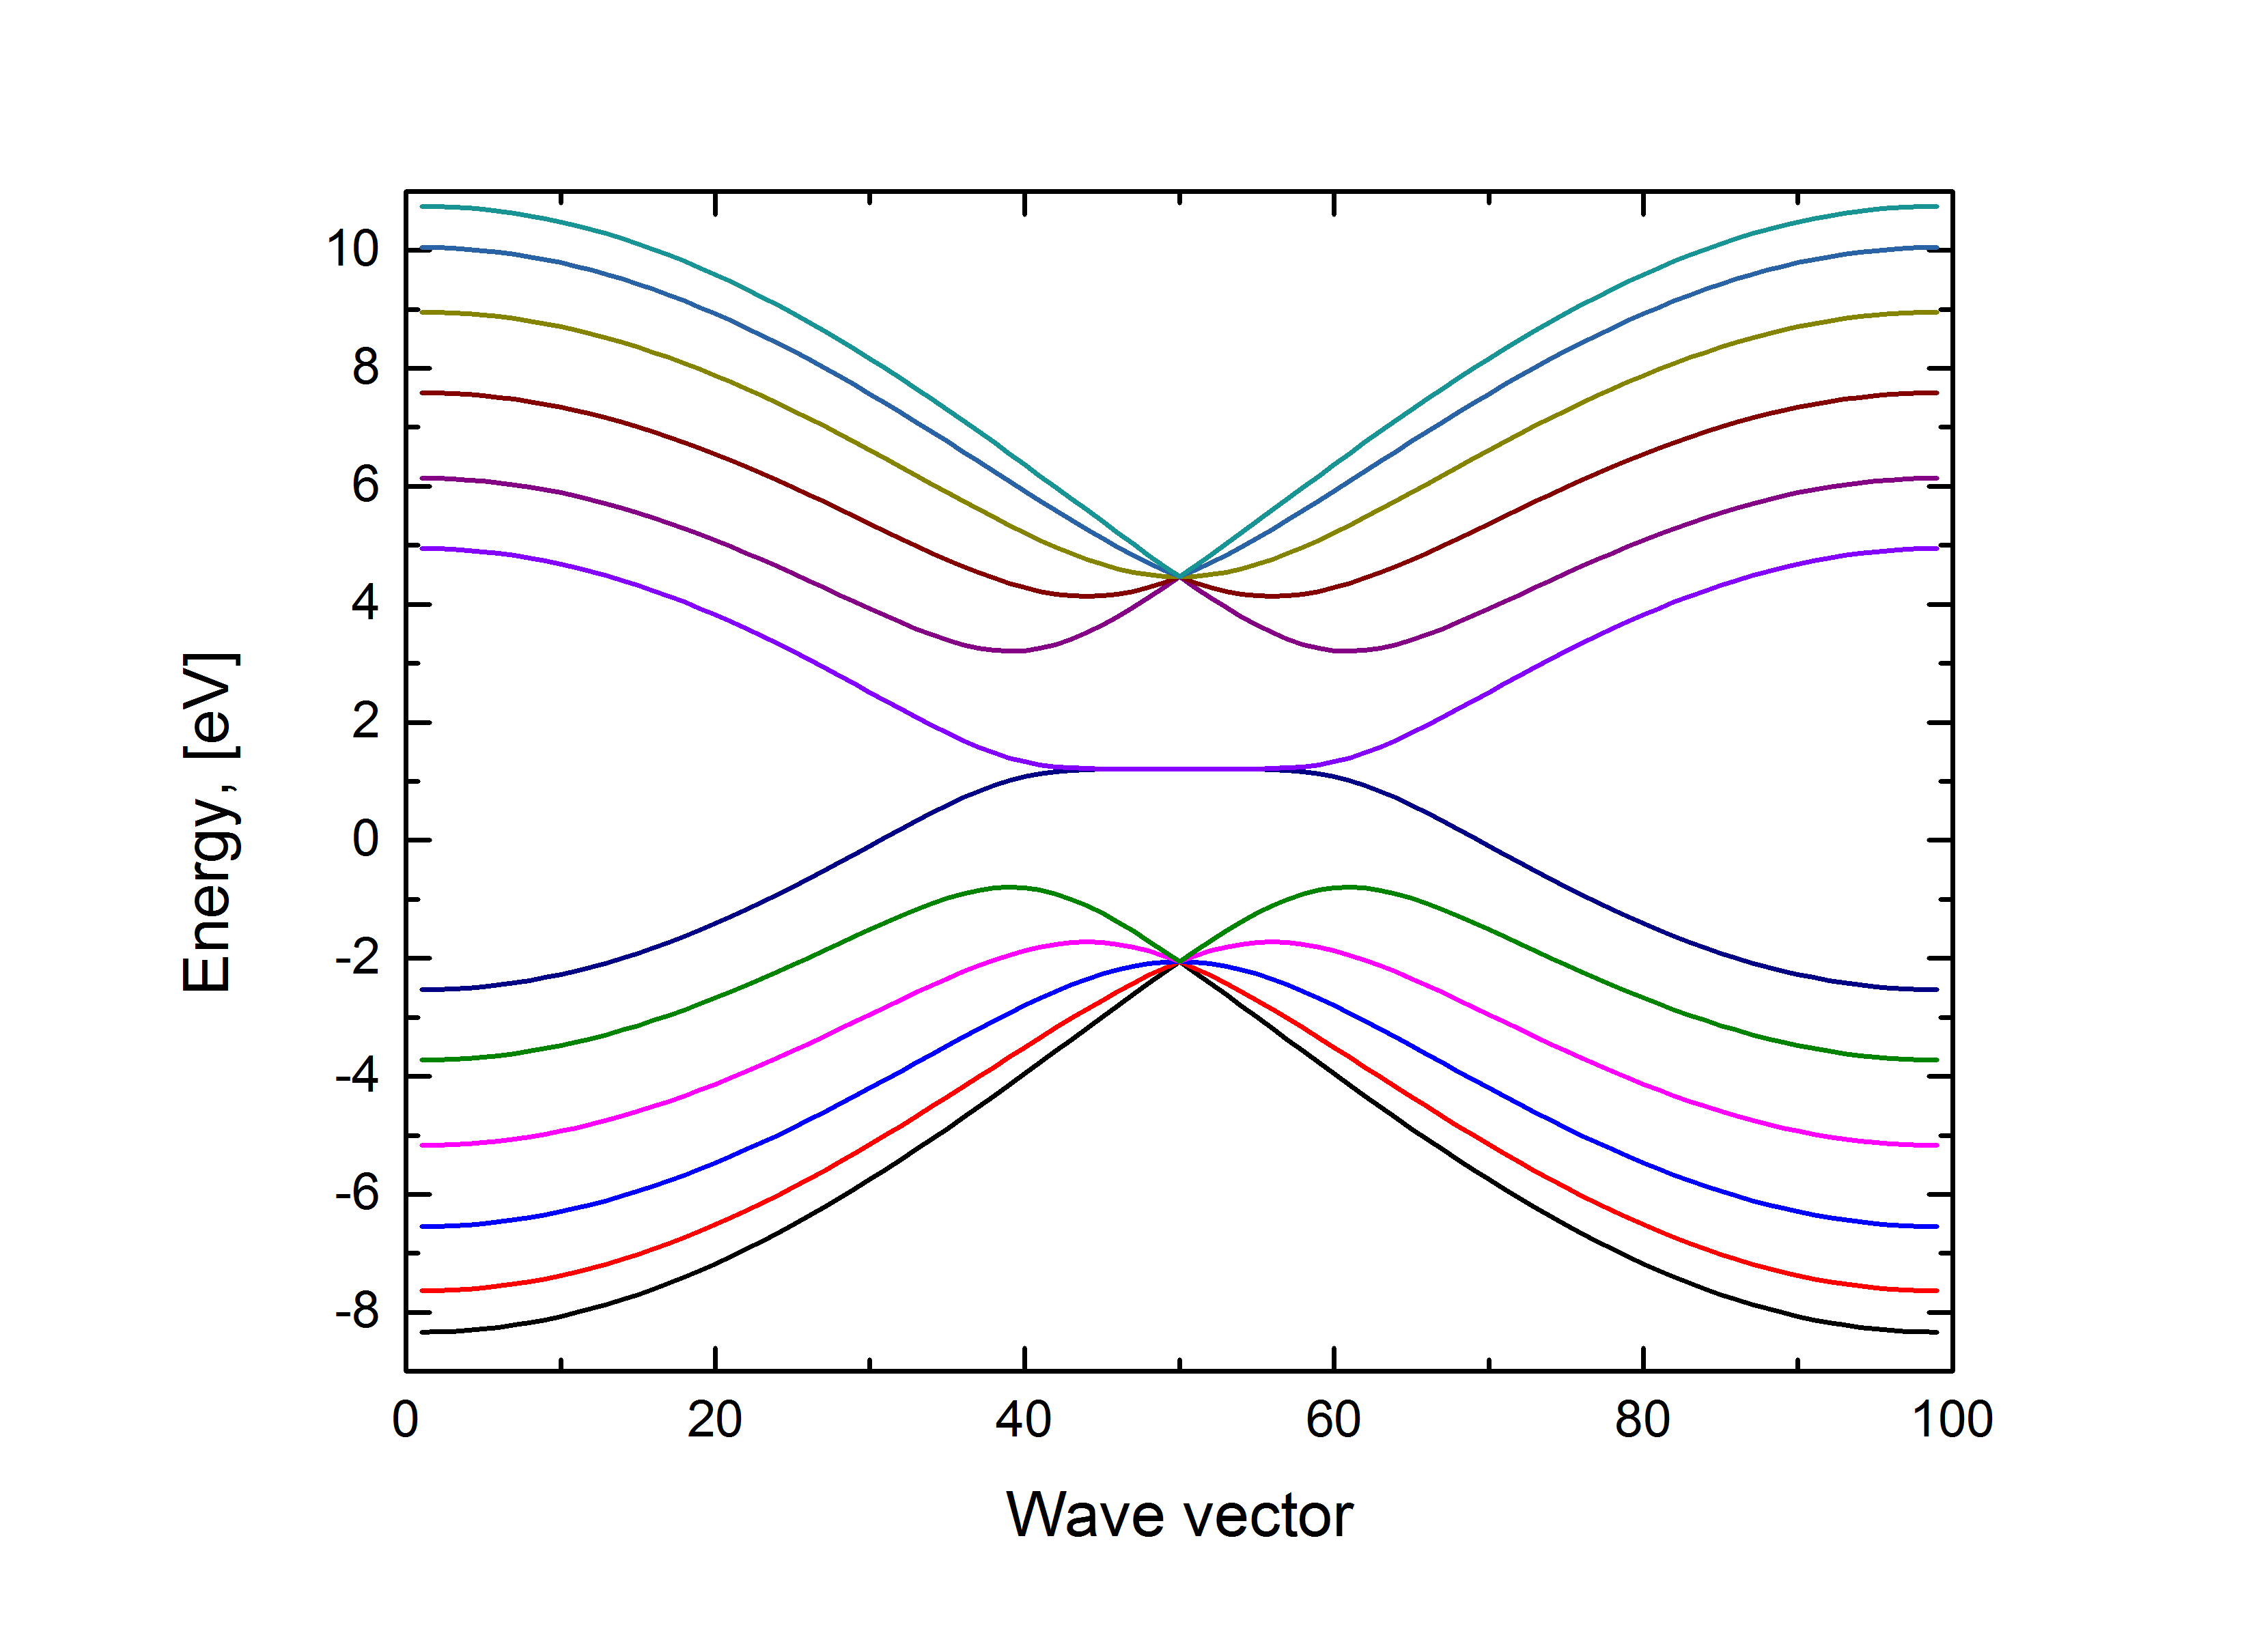
\includegraphics[width=\linewidth]{img/zz_ribbon_6}
  \caption{$n=6$}
  \label{fig:zz6}
\end{subfigure}
\begin{subfigure}{.5\textwidth}
  \centering
  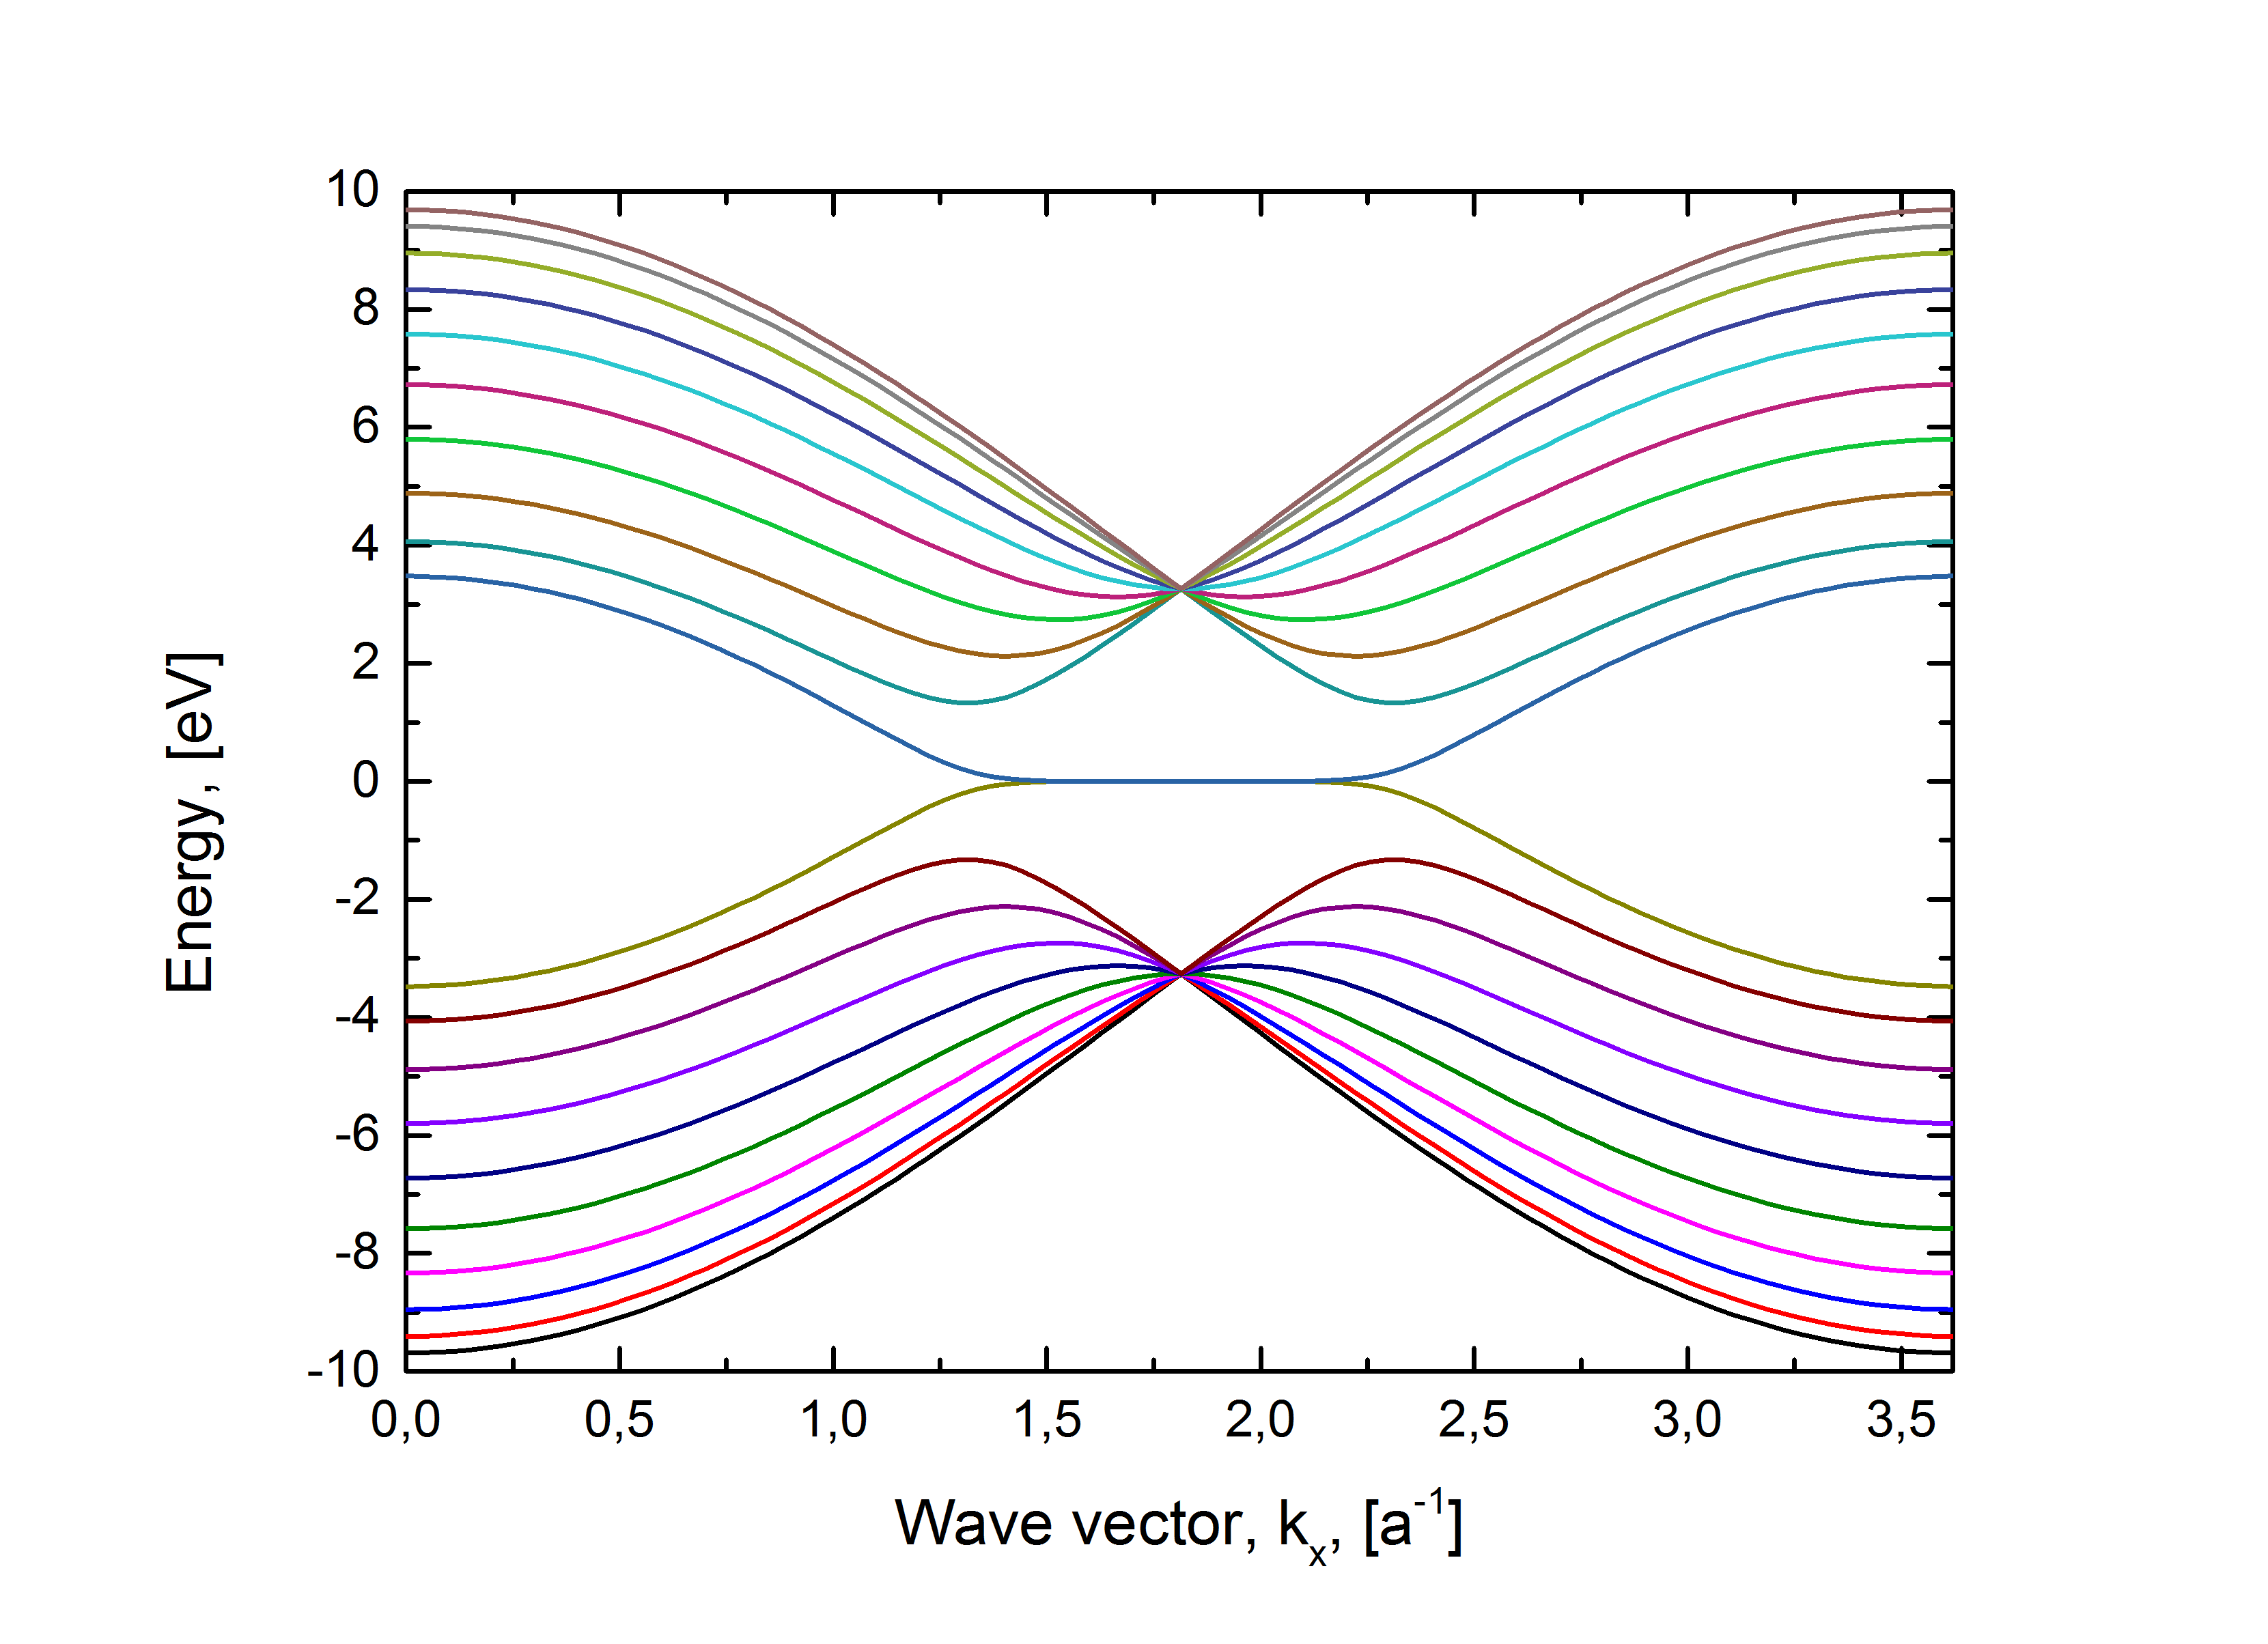
\includegraphics[width=\linewidth]{img/zz_ribbon_10}
  \caption{$n=10$}
  \label{fig:zz10}
\end{subfigure}%
\begin{subfigure}{.5\textwidth}
  \centering
  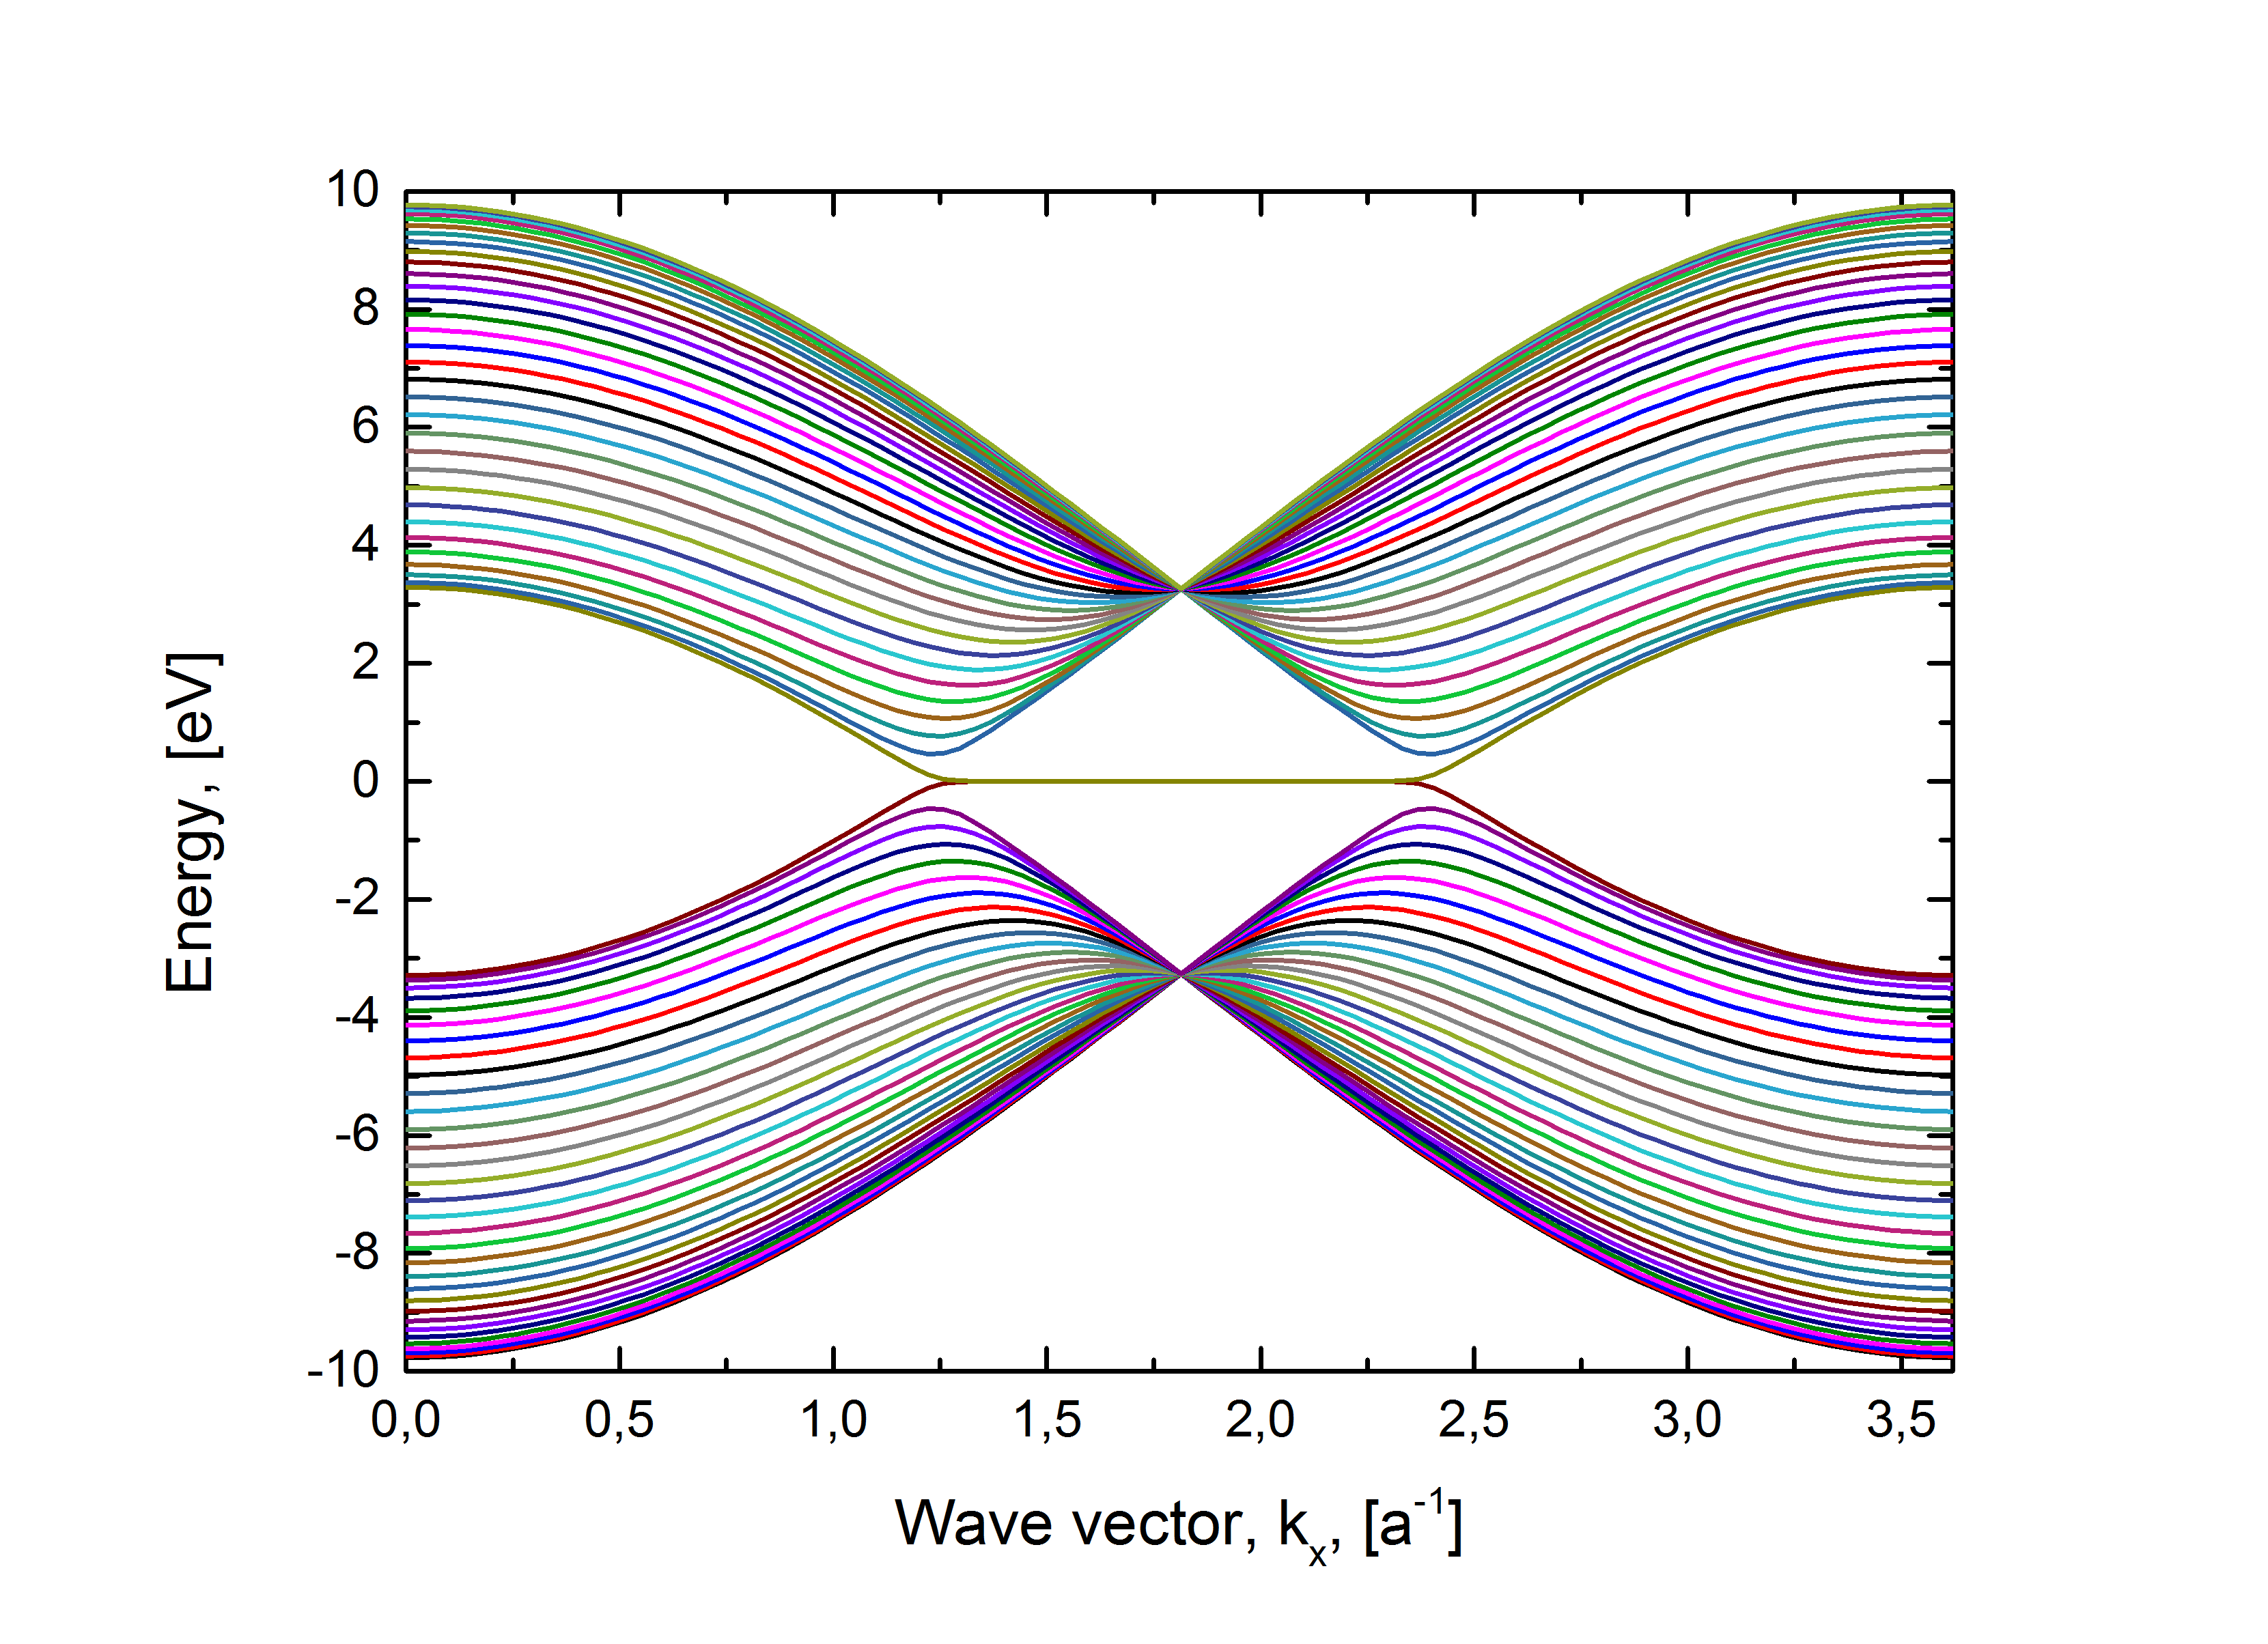
\includegraphics[width=\linewidth]{img/zz_ribbon_32}
  \caption{$n=32$}
  \label{fig:zz32}
\end{subfigure}
\begin{subfigure}{.5\textwidth}
  \centering
  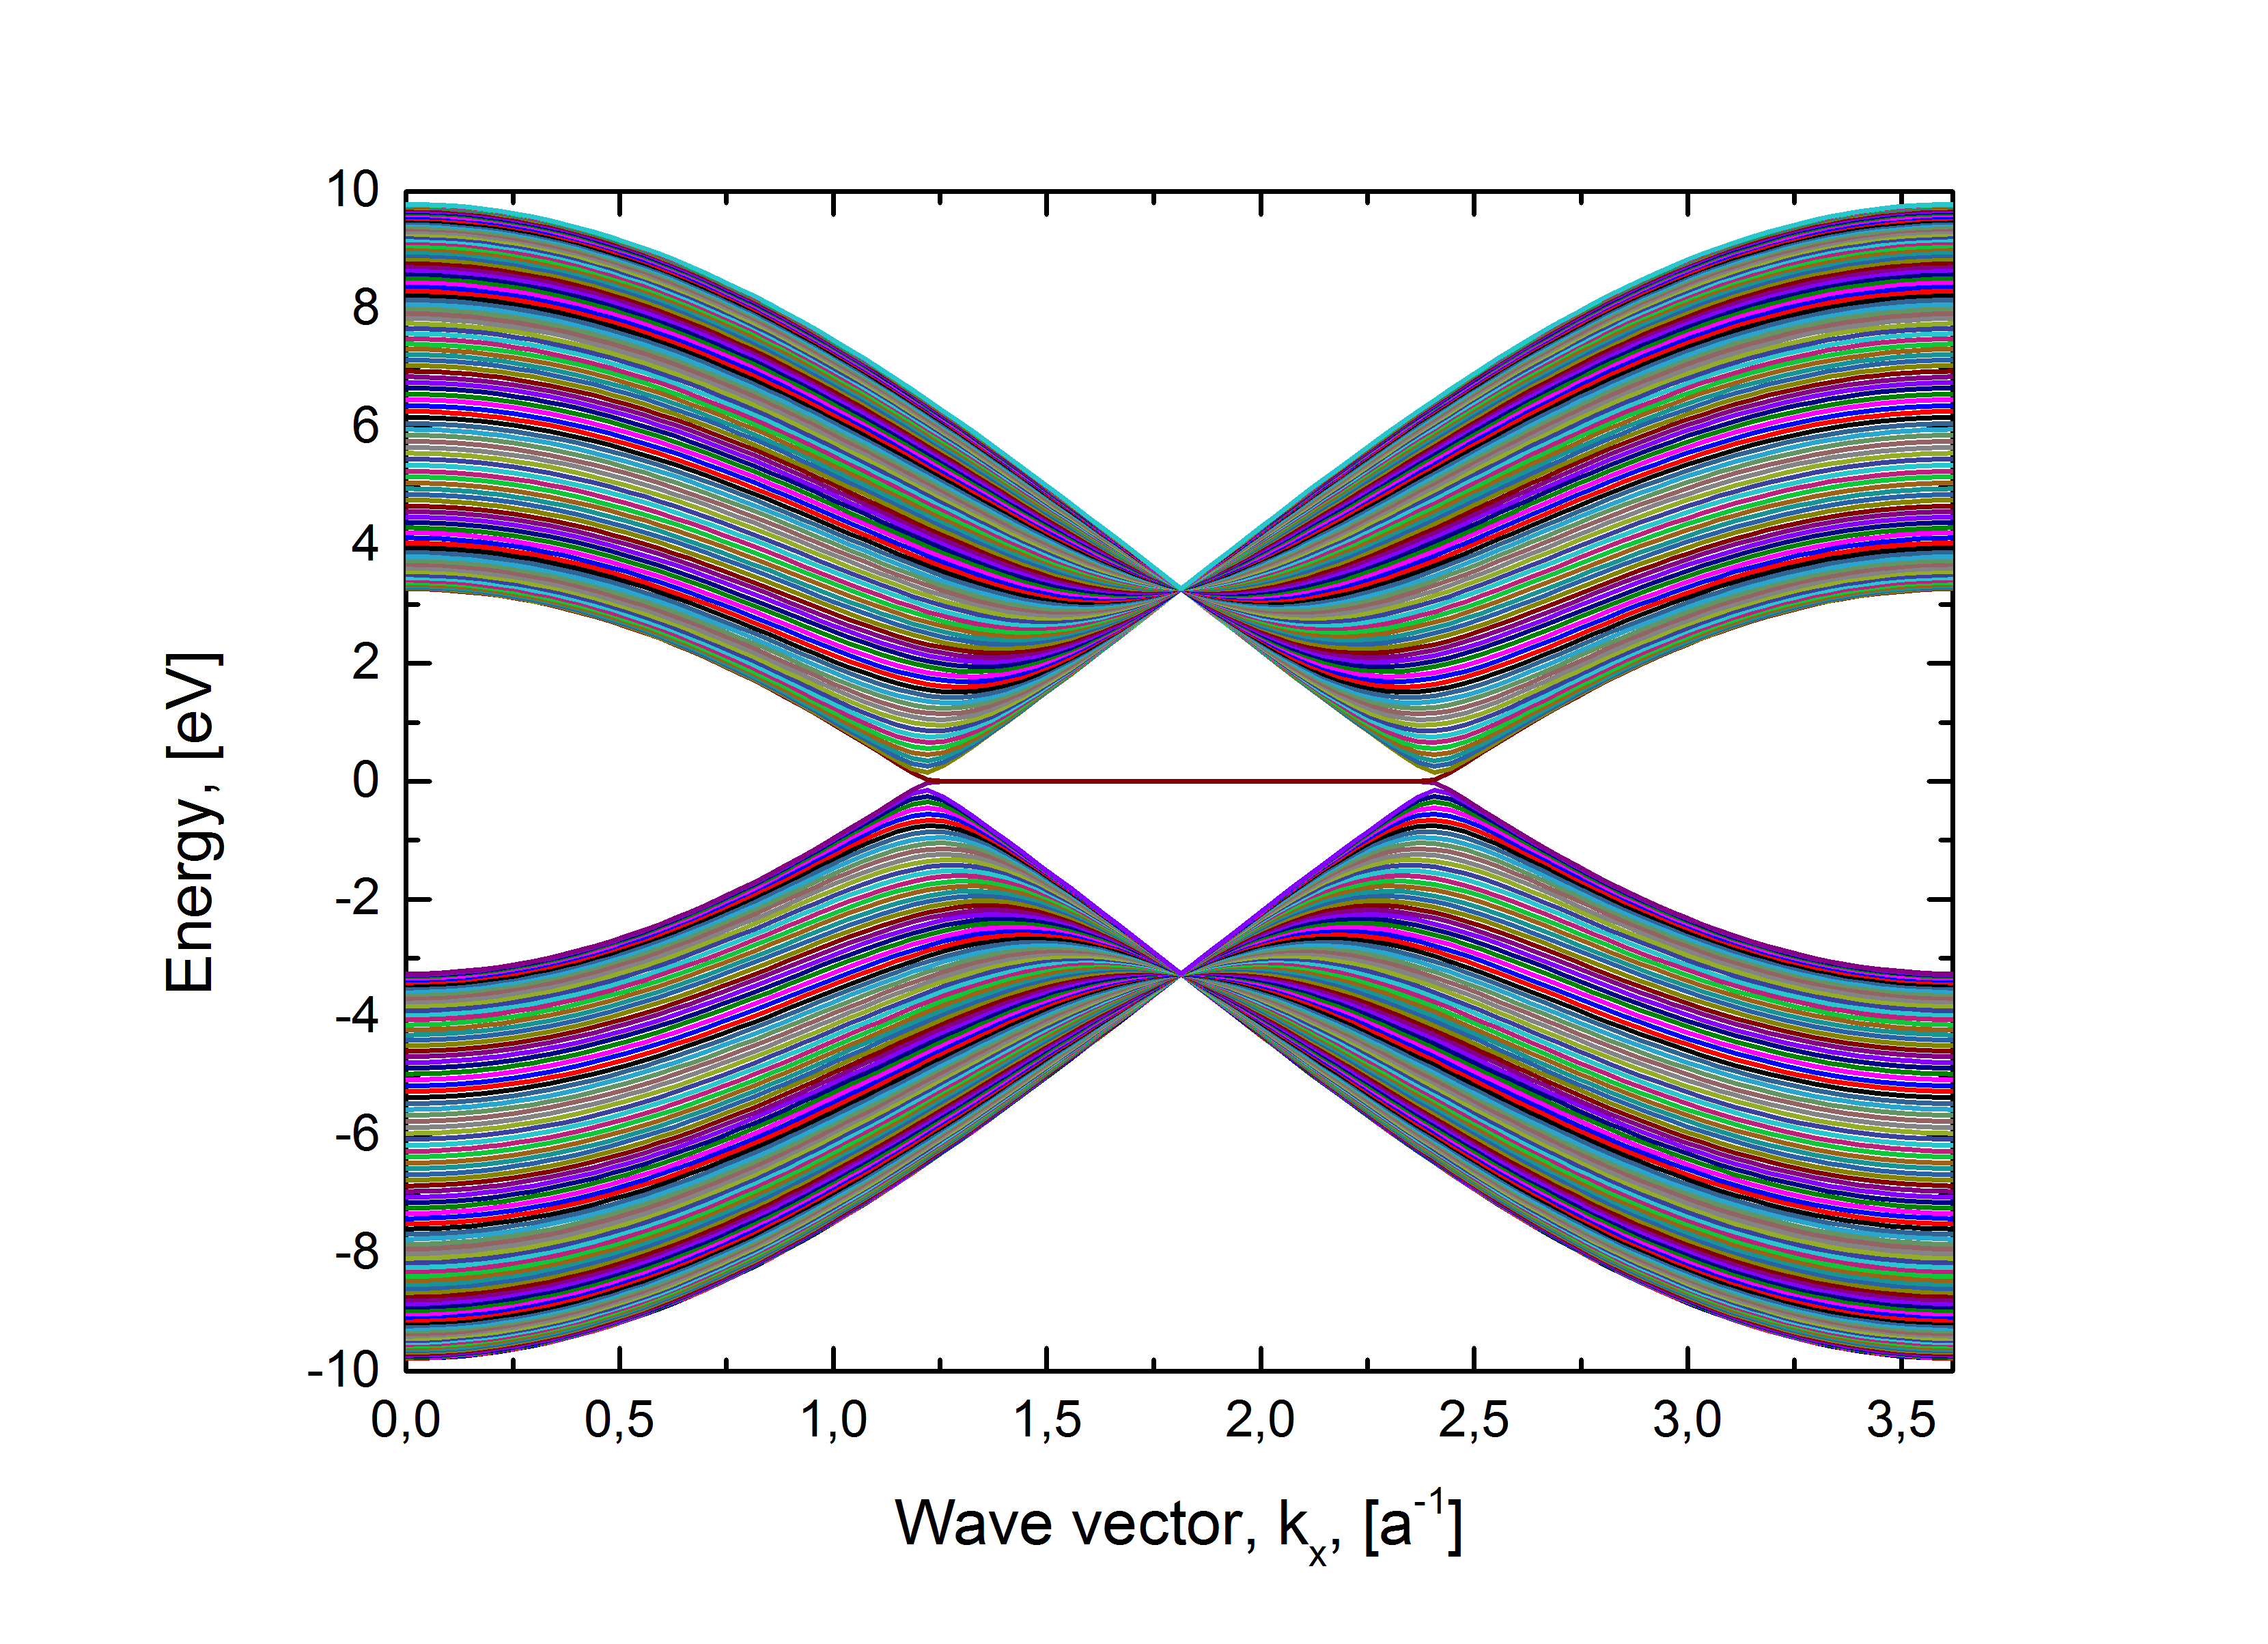
\includegraphics[width=\linewidth]{img/zz_ribbon_100}
  \caption{$n=100$}
  \label{fig:zz100}
\end{subfigure}
\caption{Calculated band structure of zigzag nanoribbons of various widths $n$ atoms.\label{fig:zz_ribbons}}
\end{figure}
